% !TEX root = ../main.tex
\chapter{Fluidfysikk}
\label{Chapter:fluiddynamikk}
\intro{Så langt har vi stort sett sett på faste legemer: klosser, biler, bjelker og stiger. Men mye av verden rundt oss består av stoffer som flyter — vann, olje og luft. Slike stoffer kaller vi \emph{fluider}. I dette kapitlet skal vi innføre to nye størrelser, massetetthet og trykk, og se hvordan trykket i en væske øker jo dypere vi kommer. Deretter skal vi se hvordan en liten kraft kan løfte en bil (Pascals lov), og hvorfor noen ting flyter mens andre synker (Arkimedes' lov).}

\spm{}{%
\item Hva er et fluid, og hva skiller det fra et fast stoff?
\item Hva bestemmer trykket i en væske?
\item Hvordan kan en liten kraft løfte en bil?
\item Hva er oppdrift, og hvorfor flyter noen ting mens andre synker?}
\newpage

\section{Introduksjon til Fluidfysikk}

\begin{wrapfigure}[6]{r}[1.5cm]{3.6cm}
\vspace{-\baselineskip}%
\rotatebox{-15}{\href{https://youtu.be/yae_lrRpSNM?si=wnCO-6XRPvQMeHbb}{%
\begin{tikzpicture}[inner sep=0pt]
\node[anchor=south west] (thumb) at (0,0) {
\includegraphics[width=3.6cm]{Images/YouTubeLenker/YT_Fluidmekanikk.png}};
\node[anchor=north west] at (thumb.south west) {
\includegraphics[width=1.2cm]{Images/YouTubeLenker/Icon.png}};
\end{tikzpicture}%
}}%
\end{wrapfigure}

Fluidfysikk handler om studiet av fluider, som inkluderer både væsker og gasser. Et fluid er et materiale som kan flyte og tilpasse seg formen til beholderen det er i. I motsetning til faste stoffer, som har en fast form og volum, kan fluider lett endre form og tilpasse seg omgivelsene.\\

Væsker, som vann, har gjerne et bestemt volum, men kan flyte og tilpasse seg formen til beholderen sin. De har høyere tetthet enn gasser, og molekylene i en væske er relativt tettpakket, men de kan fortsatt bevege seg rundt hverandre. Gasser, som luft, har verken en fast form eller et fast volum. Gasser vil utvide seg og fylle hele volumet til beholderen de er i, og molekylene i en gass har mye større bevegelsesfrihet enn i en væske.

\subsection{Massetetthet}

Massetetthet er et mål på hvor mye masse som er pakket inn i et gitt volum av et stoff. Tettheten varierer mellom forskjellige materialer. For eksempel har metall en høyere tetthet enn tre.
\tanke{}{Skip med skrog laget av metall flyter, enda metall er tyngre enn vann. Kan du forklare hvorfor?}

Tetthet er en viktig egenskap i både fysikk og ingeniørfag og måles naturligvis i kg/m\(^3\) eller g/cm\(^3\).

\defn{Massetetthet}{
    Massetetthet \( \rho \) kan uttrykkes som:
    \begin{align}
        \rho = \frac{m}{V}
    \end{align}
    hvor \( m \) er massen til stoffet og \( V \) er volumet. Massetettheten angir hvor mye masse som finnes per volumenhet.
}


\begin{table}[h!]
    \centering
    \begin{tabular}{|c|c|}
        \hline
        \textbf{Stoff} & \textbf{Tetthet \( \rho \) (\(10^3\) kg/m\(^3\))} \\
        \hline
        Gull & 19.3 \\
        \hline
        Kvikksølv & 13.6 \\
        \hline
        Stål & 7.85 \\
        \hline
        Aluminium & 2.70 \\
        \hline
        Sjøvann & 1.03 \\
        \hline
        Vann & 1.0 \\
        \hline
        Is & 0.92 \\
        \hline
        Luft & 0.0012 \\
        \hline
        Vanndamp & 0.0006 \\
        \hline
    \end{tabular}
    \caption{Massetetthet \( \rho \) til forskjellige stoffer, angitt i \( 10^3 \) kg/m\(^3\).}
    \label{tab:massetetthet}
\end{table}

\exm{Massen til en liter vann}{%
Hva er massen til \SI{1.0}{\litre} vann?
}

\svar{%
Vi vet at massetetthet \( \rho \) er definert som massen \( m \) per volum \( V \):
\[
\rho = \frac{m}{V}
\]
For å finne massen \( m \), omformer vi formelen slik at
\[
m = \rho \cdot V
\]

Siden vi har oppgitt volumet som \( V = 1.0 \, \text{L} \), konverterer vi dette til kubikkmeter:
\[
1.0 \, \text{L} = 1.0 \, \text{dm}^3 = 1.0 \cdot 10^{-3} \, \text{m}^3
\]

Nå setter vi inn verdiene med \( \rho = 1.0 \cdot 10^3 \, \text{kg/m}^3 \) (tabell~\ref{tab:massetetthet}) og \( V = 1.0 \cdot 10^{-3} \, \text{m}^3 \):
\[
m = (1.0 \cdot 10^3 \, \text{kg/m}^3) \cdot (1.0 \cdot 10^{-3} \, \text{m}^3)
  = \doubleunderline{1.0 \, \text{kg}}
\]
Én liter vann har altså en masse på omtrent ett kilogram. Dette er lurt å huske, fordi det gjør det lett å anslå massen til vann i bøtter, flasker og badekar.
}

\oppgaver{Hvilket metall?}{k7oppg1}{%
%
En liten metallterning har sidekanter på \SI{3.0}{\centi\metre} og masse \SI{73}{\gram}.
\begin{enumerate}[a)]
    \item Finn volumet til terningen i \si{\centi\metre\cubed} og i \si{\metre\cubed}.
    \item Finn massetettheten til terningen. Bruk tabell~\komplabel{tab:massetetthet} til å finne ut hvilket metall terningen sannsynligvis er laget av.
    \item Hvor stor masse ville en like stor terning av gull hatt?
\end{enumerate}
%
%
}


\subsection{Trykk}

Trykk er definert som kraften som virker vinkelrett på en overflate per arealenhet. Det beskriver hvor mye kraft som påføres en bestemt flate. Trykk måles ofte i enheter av pascal (Pa), hvor \( 1 \, \text{Pa} = 1 \, \text{N/m}^2 \).

\defn{Trykk}{
    Trykket \( p \) er gitt ved:
    \begin{align}
        p = \frac{F}{A}
    \end{align}
    hvor \( F \) er kraften som virker vinkelrett på overflaten, og \( A \) er arealet til overflaten. Trykk måler kraft per arealenhet og uttrykkes vanligvis i pascal (Pa).
Dette betyr at trykk også kan uttrykkes som \( 1 \, \text{Pa} = 1 \, \text{kg} \cdot \text{m}^{-1} \cdot \text{s}^{-2} \).}

Trykk er en skalar størrelse. Det betyr at trykk kun har en størrelse, men ingen retning. Trykk er altså IKKE en vektor! Det er \emph{kraften} fra trykket som har en retning: den står alltid vinkelrett på flaten den virker på.\\

Formelen $p = F/A$ forteller oss at den samme kraften kan gi svært ulikt trykk, avhengig av hvor stort areal kraften fordeles over. Det skal vi se i neste eksempel.

\exm{Ski eller støvler?}{%
En person med masse $m = \SI{72}{\kilo\gram}$ står på snø. Vi antar at trykket er jevnt fordelt over støvelsålene.
\begin{enumerate}[a)]
    \item Finn trykket mot snøen når personen står i støvler. Til sammen har de to sålene et areal på $A = \SI{0.050}{\metre\squared}$.
    \item Personen tar på seg ski. Hver ski er \SI{1.8}{\metre} lang og \SI{7.0}{\centi\metre} bred. Finn trykket mot snøen nå (anta at skiene er uendelig stive, slik at trykket blir jevnt fordelt).
    \item Forklar hvorfor det er lettere å gå i dyp snø med ski enn med støvler.
\end{enumerate}
}

\svar{%
\noindent
Kraften som virker vinkelrett på snøen, er tyngden av personen:
\[
    F = m\mathrm{g} = \SI{72}{\kilo\gram}\cdot\SI{9.81}{\metre\per\second\squared} = \SI{706.3}{\newton}
\]

\smallskip\noindent
\textbf{a)} Med støvler fordeles kraften over $A = \SI{0.050}{\metre\squared}$:
\[
    p = \frac{F}{A} = \frac{\SI{706.3}{\newton}}{\SI{0.050}{\metre\squared}} = \SI{14126}{\pascal} \approx \doubleunderline{\SI{14}{\kilo\pascal}}
\]

\smallskip\noindent
\textbf{b)} Med ski er arealet
\[
    A = 2\cdot \SI{1.8}{\metre}\cdot\SI{0.070}{\metre} = \SI{0.252}{\metre\squared},
\]
og trykket blir
\[
    p = \frac{\SI{706.3}{\newton}}{\SI{0.252}{\metre\squared}} = \SI{2803}{\pascal} \approx \doubleunderline{\SI{2.8}{\kilo\pascal}}
\]

\smallskip\noindent
\textbf{c)} Kraften mot snøen er like stor i begge tilfeller. Men med ski fordeles kraften over et omtrent fem ganger så stort areal, og da blir trykket omtrent fem ganger så lite. Snøen blir derfor ikke presset like mye sammen, og man synker mindre ned.
}

På mikroskopisk nivå er trykk en konsekvens av interaksjoner. Se for deg en beholder med gassmolekyler. Hvert molekyl i gassen utøver en liten kraft på veggen i beholeren hver gang det treffer den, og summen av alle disse kollisjonene per arealenhet gir opphav til trykket i beholderen. Kreftene som påføres veggen skyldes altså impulsoverføringen fra molekylene til veggen. Jo flere molekyler som treffer veggen per tidsenhet, og jo raskere de beveger seg, desto større blir trykket.

\begin{figure}[H]
    \centering
    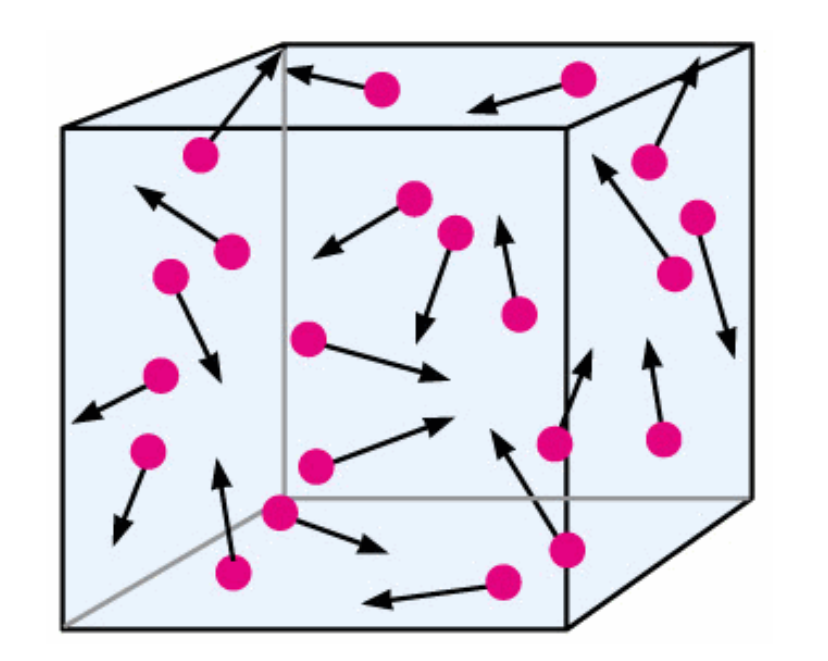
\includegraphics[width=0.6\textwidth]{Images/Kapittel4:Fluiddynamikk/Trykk.png}
    \caption{Trykk i gassbeholder}
    \label{fig:Trykk}
    \end{figure}

\oppgaver{Tegnestift}{k7oppg2}{%
%
Du trykker en tegnestift inn i en vegg med tommelen. Kraften fra tommelen på stiften er $F = \SI{20}{\newton}$. Hodet på tegnestiften har areal \SI{1.0}{\centi\metre\squared}, og spissen har areal \SI{0.10}{\milli\metre\squared}.
\begin{enumerate}[a)]
    \item Finn trykket mot tommelen.
    \item Stiften er i ro i det øyeblikket du trykker, så den presser på veggen med den samme kraften. Finn trykket fra spissen mot veggen.
    \item Forklar hvorfor stiften går inn i veggen, men ikke inn i tommelen.
\end{enumerate}
\textit{Hint: Husk at $\SI{1}{\centi\metre\squared} = \SI{1e-4}{\metre\squared}$ og $\SI{1}{\milli\metre\squared} = \SI{1e-6}{\metre\squared}$.}
%
%
}

\subsection{Lufttrykk}
\tanke{}{Hvorfor fungerer sugekopper?}

Her nede på jordens overflate er vi mennesker omgitt av luft. Det vi kanskje ikke tenker på, er at denne luften veier noe. Den har vekt. Når du stiger ned i vann, merker du at vannet utøver et trykk på deg. Det er på grunn av vannets vekt. Men luften gjør det samme. Lufttrykket rundt oss (som følge av luftens vekt) er omtrent \SI{1.013e5}{\pascal}. Dette trykket kalles også \emph{én atmosfære} (1 atm).
\graabox{$\displaystyle 1\,\text{atm} = \SI{101325}{\pascal} \approx \SI{1.013e5}{\pascal}$}

\begin{wrapfigure}[6]{r}[1.5cm]{3.6cm}
\vspace{-\baselineskip}%
\rotatebox{-15}{\href{https://www.nrk.no/video/132654}{%
\begin{tikzpicture}[inner sep=0pt]
\node[anchor=south west] (thumb) at (0,0) {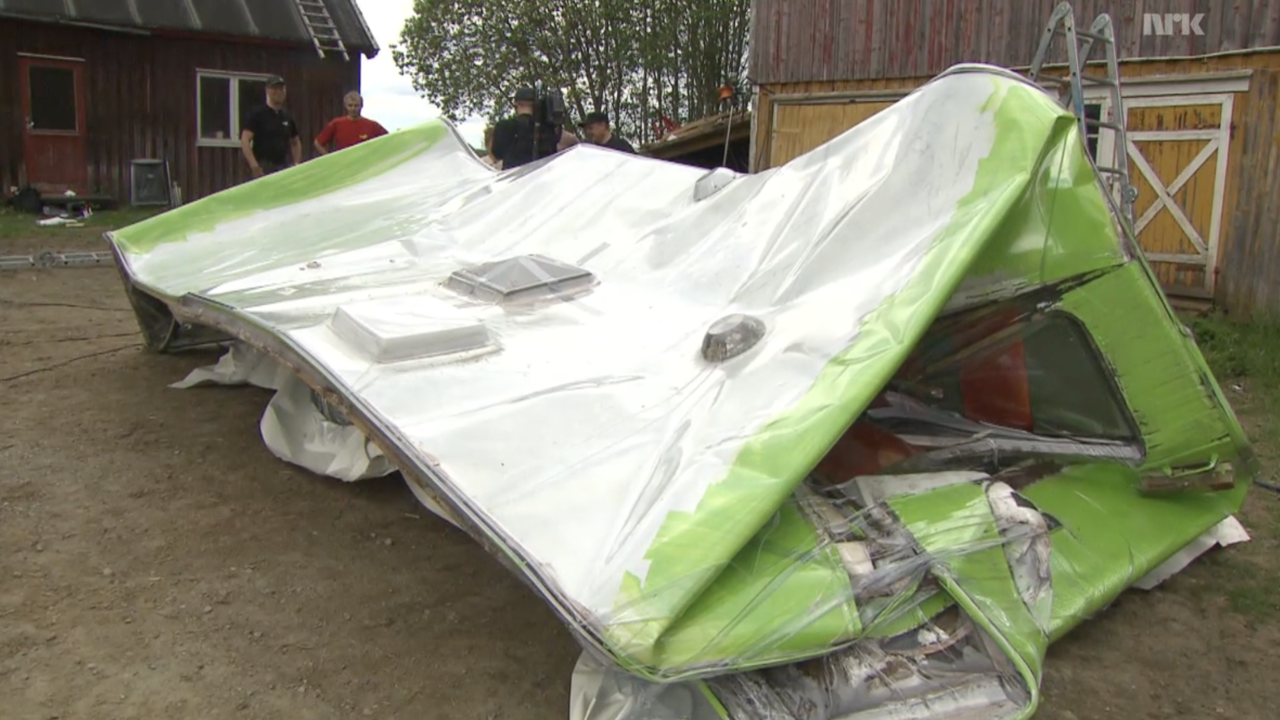
\includegraphics[width=3.6cm]{Images/YouTubeLenker/NRK_Campingvogn.png}};
\fill[black, opacity=0.55] (thumb.center) circle (0.42cm);
\draw[white, line width=1.2pt] (thumb.center) circle (0.42cm);
\fill[white] ($(thumb.center)+(-0.13,-0.2)$) -- ($(thumb.center)+(-0.13,0.2)$) -- ($(thumb.center)+(0.22,0)$) -- cycle;
\node[anchor=north west, font=\scriptsize\bfseries, text=black!75] at ([yshift=-2pt]thumb.south west) {Videoklipp};
\end{tikzpicture}%
}}%
\end{wrapfigure}
Grunnen til at sugekopper fungerer, er trykket fra luften. Lufttrykket tvinger sugekoppen til å holde seg på plass. Desto større flate sugekoppen har, desto større blir de totale kreftene som holder den på plass. Det er derfor sugekopper med større diameter holder bedre enn små sugekopper. Dette betyr at dersom du pumper vekk luften fra et rom, vil alt som er festet med sugekopper slippe taket, fordi det ikke lenger er lufttrykk som holder dem på plass.

Lufttrykket virker fra alle kanter på alt som er omgitt av luft. Siden \SI{1}{atm} er et stort trykk, kan kraften fra lufta bli svært stor, selv på helt vanlige flater. I videoklippet (fra NRK) ser du hva som skjer med en campingvogn når lufta inni den pumpes ut. Hvor store krefter det er snakk om, ser vi i neste eksempel.
\WFclear

\exm{Lufta presser på et bord}{%
Et bord har en rektangulær bordplate som er \SI{1.2}{\metre} lang og \SI{0.80}{\metre} bred. Lufttrykket er $p_0 = \SI{1.013e5}{\pascal}$.
\begin{enumerate}[a)]
    \item Finn kraften fra lufta på oversiden av bordplata.
    \item Hvor stor masse ville hatt en like stor tyngde?
    \item Hvorfor knekker ikke bordet sammen?
\end{enumerate}
}

\svar{%
\noindent
\textbf{a)} Arealet av bordplata er
\[
    A = \SI{1.2}{\metre}\cdot\SI{0.80}{\metre} = \SI{0.96}{\metre\squared}
\]
Fra definisjonen av trykk, $p = F/A$, er kraften fra lufta
\[
    F = p_0 A = \SI{1.013e5}{\pascal}\cdot\SI{0.96}{\metre\squared} = \SI{9.72e4}{\newton} \approx \doubleunderline{\SI{9.7e4}{\newton}}
\]

\smallskip\noindent
\textbf{b)} En masse $m$ har tyngden $m\mathrm{g}$. Vi setter $m\mathrm{g} = F$:
\[
    m = \frac{F}{\mathrm{g}} = \frac{\SI{9.72e4}{\newton}}{\SI{9.81}{\metre\per\second\squared}} = \SI{9.91e3}{\kilo\gram} \approx \doubleunderline{\SI{9.9e3}{\kilo\gram}}
\]
Lufta presser altså på bordplata med en kraft som tilsvarer tyngden av nesten ti tonn!

\smallskip\noindent
\textbf{c)} Lufta presser ikke bare på oversiden av bordplata, men også på undersiden, med det samme trykket. Kraften oppover på undersiden er derfor like stor som kraften nedover på oversiden, og de to kreftene opphever hverandre. Bordet merker bare tyngden av det som ligger på det.
}

Inne i et bildekk er trykket større enn lufttrykket utenfor. Trykkmålere på bensinstasjonen viser \emph{overtrykket}, altså hvor mye større trykket i dekket er enn lufttrykket rundt. Dekktrykk oppgis ofte i enheten bar, der $\SI{1}{bar} = \SI{1.0e5}{\pascal}$.

\exm{Lufttrykk i bildekk}{%
En trykkmåler viser at overtrykket i et bildekk er \SI{2.3}{bar}, altså $\SI{2.3e5}{\pascal}$. Lufttrykket utenfor er $p_0 = \SI{1.013e5}{\pascal}$.
\begin{enumerate}[a)]
    \item Finn det totale trykket inne i dekket. Hvor mange atmosfærer er det?
    \item Bilen har masse \SI{1200}{\kilo\gram}, og vi antar at tyngden fordeler seg likt på de fire hjulene. Det er overtrykket i dekket som bærer bilen. Hvor stort areal av hvert dekk må ligge an mot veien? Vi ser bort fra stivheten i dekkveggen.
\end{enumerate}
}

\svar{%
\noindent
\textbf{a)} Det totale trykket er lufttrykket pluss overtrykket:
\[
    p = p_0 + \Delta p = \SI{1.013e5}{\pascal} + \SI{2.3e5}{\pascal} = \SI{3.31e5}{\pascal} \approx \doubleunderline{\SI{3.3e5}{\pascal}}
\]
Målt i atmosfærer er dette
\[
    \frac{\SI{3.31e5}{\pascal}}{\SI{1.013e5}{\pascal}} = 3.27 \approx \doubleunderline{\SI{3.3}{atm}}
\]

\smallskip\noindent
\textbf{b)} Hvert hjul bærer en fjerdedel av tyngden:
\[
    F = \frac{m\mathrm{g}}{4} = \frac{\SI{1200}{\kilo\gram}\cdot\SI{9.81}{\metre\per\second\squared}}{4} = \SI{2943}{\newton}
\]
Der dekket ligger an mot veien, presser lufta inne i dekket nedover med trykket $p_0 + \Delta p$, mens lufta utenfor bare presser med $p_0$. Det er altså overtrykket $\Delta p$ som gir nettokraften som bærer bilen: $F = \Delta p\cdot A$. Dermed er
\[
    A = \frac{F}{\Delta p} = \frac{\SI{2943}{\newton}}{\SI{2.3e5}{\pascal}} = \SI{1.28e-2}{\metre\squared} \approx \doubleunderline{\SI{1.3e-2}{\metre\squared}}
\]
Det tilsvarer omtrent \SI{130}{\centi\metre\squared}, eller en flate på omtrent $\SI{11}{\centi\metre}\times\SI{11}{\centi\metre}$. Har dekket for lavt trykk, må en større del av dekket ligge an mot veien for å bære bilen. Dekket blir da flatere, og bilen bruker mer drivstoff.
}

\section{Trykk i væsker}

Trykk i væsker oppstår som følge av vekten av væsken over et gitt punkt og de kreftene som væsken utøver på overflatene rundt seg. Dette trykket avhenger av væskens tetthet \( \rho \), dybden \( h \), og tyngdeakselerasjonen \( \mathrm{g} \). Vi kan analysere væsketrykket ved å bruke to forskjellige elementer: et horisontalt væskeelement og et vertikalt væskeelement.

\subsection{Horisontalt væskeelement}
I et horisontalt væskeelement er trykket likt i alle retninger, forutsatt at væsken er i ro. Dette skyldes at væsker alltid fordeler kreftene jevnt i et horisontalt plan når de ikke er i bevegelse. Dersom trykket ikke var likt, ville væsken begynne å strømme fra områder med høyt trykk til områder med lavt trykk. Derfor gjelder:
\begin{tcolorbox}[enhanced, arc=2mm, boxrule=0pt, colframe=black!8!white, colback=black!8!white,
    top=7pt, bottom=7pt, before skip=6pt, after skip=6pt]
\centering $\displaystyle p_1 = p_2$
\end{tcolorbox}
\begin{wrapfigure}[6]{r}[1.5cm]{3.6cm}
\vspace{-\baselineskip}%
\rotatebox{-15}{\href{https://youtu.be/wLk8RaTSvn8?si=7_7LX2zwetDUtLVY}{%
\begin{tikzpicture}[inner sep=0pt]
\node[anchor=south west] (thumb) at (0,0) {
\includegraphics[width=3.6cm]{Images/YouTubeLenker/YT_Hydrostatikk1.png}};
\node[anchor=north west] at (thumb.south west) {
\includegraphics[width=1.2cm]{Images/YouTubeLenker/Icon.png}};
\end{tikzpicture}%
}}%
\end{wrapfigure}
I et horisontalt væskeelement i ro er altså trykket det samme i alle punkter på samme nivå.

Men merk at dersom væsken er i bevegelse, kan trykket variere i horisontal retning. For eksempel, i et rør hvor arealet av røret endrer seg, vil væsken strømme med ulik fart i de ulike delene av røret, med det resultat at trykket blir forskjellig. Der røret er smalt, strømmer væsken fortere, og der er trykket lavere.

\begin{figure}[H]
    \centering
    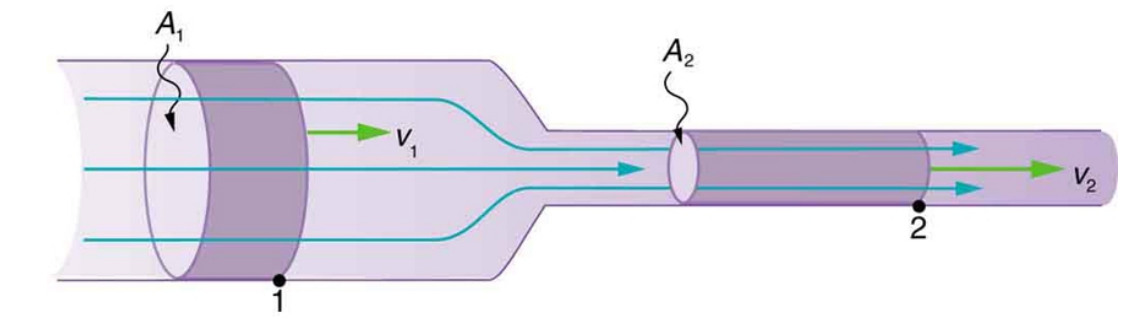
\includegraphics[width=0.8\textwidth]{Images/Kapittel4:Fluiddynamikk/rør_ulikt_trykk.png}
    \caption{Et rør der arealet reduseres fra \( A_1 \) til \( A_2 \). Væsken strømmer fortere i den smale delen av røret (\(v_2 > v_1\)), og trykket i punkt 2 er lavere enn i punkt 1. Slike scenario er ikke del av pensum i dette faget, hvor vi holder oss til fluidstatikk.}
    \label{fig:roer_variabelt_areal}
\end{figure}


I dette faget skal vi ikke studere væsker i bevegelse, slik som i eksemplet over. Vi holder oss til fluid\textit{statikken}.

\defn{Trykk i horisontalt væskeelement}{
    I et horisontalt væskeelement i ro gjelder:
    \begin{align}
        p_1 = p_2
    \end{align}
    hvor \( p_1 \) og \( p_2 \) er trykkene i forskjellige punkter på samme horisontale nivå i den samme sammenhengende væsken. Dersom væsken strømmer og rørets areal endrer seg, vil trykket kunne variere.
}

Legg merke til at definisjonen krever at punktene ligger i den \emph{samme sammenhengende} væsken. Det betyr at vi må kunne gå fra det ene punktet til det andre uten å forlate væsken. Hvor mye vann som ligger rett over hvert punkt, spiller ingen rolle. Det ser vi i neste eksempel.

\exm{Trykket i et akvarium}{%
Et akvarium er fylt med vann som står i ro. På bunnen ligger en stein med en hule, der fiskene kan gjemme seg (se figuren). Punktene A, B og C ligger alle \SI{0.30}{\metre} under vannoverflaten. Punkt C ligger inne i hula, rett under steinen. En trykkmåler viser at trykket i punkt A er \SI{1.04e5}{\pascal}.
\begin{enumerate}[a)]
    \item Hva er trykket i punkt B?
    \item Hva er trykket i punkt C, inne i hula?
    \item Punkt D ligger litt dypere enn A, B og C. Er trykket i D større eller mindre enn i A?
\end{enumerate}

\begin{center}
\begin{tikzpicture}[scale=1.0, font=\small]
  % Vann
  \fill[oppgcol!18] (0,0) rectangle (7.0,3.0);
  % Stein med overheng (hule åpen mot venstre)
  \fill[gray!45, rounded corners=4pt] (5.0,0) -- (5.0,1.4) -- (3.8,1.4) -- (3.8,1.9) -- (4.5,2.2) -- (6.2,2.25) -- (6.6,1.8) -- (6.6,0) -- cycle;
  \draw[gray!30!black, rounded corners=4pt] (5.0,0) -- (5.0,1.4) -- (3.8,1.4) -- (3.8,1.9) -- (4.5,2.2) -- (6.2,2.25) -- (6.6,1.8) -- (6.6,0);
  % Akvarium
  \draw[very thick, black!70] (0,3.5) -- (0,0) -- (7.0,0) -- (7.0,3.5);
  \draw[oppgcol!70!black, thick] (0,3.0) -- (7.0,3.0);
  % Nivålinje
  \draw[dashed, gray!70] (0,1.0) -- (7.0,1.0);
  % Punkter
  \foreach \x/\n in {1.2/A, 2.8/B, 4.4/C}{
    \fill[black] (\x,1.0) circle (2pt);
    \node[below] at (\x,1.0) {\n};
  }
  \fill[black] (2.0,0.35) circle (2pt);
  \node[right] at (2.0,0.35) {D};
  % Dybde
  \draw[<->, thin, gray!70!black] (-0.4,3.0) -- (-0.4,1.0)
      node[midway, left, font=\footnotesize] {\SI{0.30}{\metre}};
  \draw[gray!50, thin] (-0.5,1.0) -- (0,1.0);
  \draw[gray!50, thin] (-0.5,3.0) -- (0,3.0);
\end{tikzpicture}
\captionof{figure}{Et akvarium med en stein med hule. Punktene A, B og C ligger på samme dybde. Figuren er ikke i målestokk.}
\label{fig:akvarium_hule}
\end{center}
}

\svar{%
\noindent
\textbf{a)} Punktene A og B ligger på samme horisontale nivå i den samme vannmassen, og vannet er i ro. Da er trykket likt:
\[
    p_B = p_A = \doubleunderline{\SI{1.04e5}{\pascal}}
\]

\smallskip\noindent
\textbf{b)} Det ligger mindre vann rett over punkt C enn over punkt A, fordi steinen er i veien. Likevel kan vi gå fra A til C gjennom vannet, inn i hula, uten å forlate vannet. Punktene ligger altså på samme nivå i den samme sammenhengende væsken, og derfor er
\[
    p_C = p_A = \doubleunderline{\SI{1.04e5}{\pascal}}
\]
Vi kan også forstå dette slik: Hvis trykket i C var lavere enn i A, ville vannet begynt å strømme fra A inn i hula. Men vannet er i ro, så trykket må være likt.

\smallskip\noindent
\textbf{c)} Punkt D ligger dypere enn A. Da er det mer vann over D som presser nedover, og trykket i D er \doubleunderline{større} enn i A. Hvor mye større, skal vi finne ut i neste delkapittel.
}

\oppgaver{Vannkanne}{k7oppg3}{%
%
En vannkanne er fylt med vann som står i ro. Punkt A ligger inne i kanna, og punkt B ligger i tuten, i samme høyde som A (se figuren).

\begin{center}
\begin{tikzpicture}[scale=0.9, font=\small]
  % Vann (klippes ved vannflaten y = 2.4)
  \begin{scope}
    \clip (-1,-1) rectangle (5,2.4);
    \fill[oppgcol!18] (0,0) rectangle (2.4,3.0);
    \fill[oppgcol!18] (2.35,0.3) -- (3.75,3.0) -- (3.15,3.0) -- (2.35,1.5) -- cycle;
  \end{scope}
  \draw[oppgcol!70!black, thick] (0,2.4) -- (2.4,2.4);
  \draw[oppgcol!70!black, thick] (2.85,2.4) -- (3.45,2.4);
  % Kanne
  \draw[very thick, black!75] (0,3.0) -- (0,0) -- (2.4,0) -- (2.4,0.3) -- (3.75,3.0);
  \draw[very thick, black!75] (2.4,3.0) -- (2.4,1.5) -- (3.15,3.0);
  % Hank
  \draw[very thick, black!75] (0,2.6) .. controls (-0.9,2.6) and (-0.9,0.8) .. (0,0.8);
  % Punkter
  \draw[dashed, gray!70] (0.6,1.8) -- (2.85,1.8);
  \fill[black] (1.0,1.8) circle (2pt) node[below] {A};
  \fill[black] (2.85,1.8) circle (2pt) node[right=4pt] {B};
\end{tikzpicture}
\end{center}

\begin{enumerate}[a)]
    \item En trykkmåler viser at trykket i A er \SI{1.05e5}{\pascal}. Hva er trykket i B? Begrunn svaret.
    \item Bruk svaret i a) til å forklare hvorfor vannet i tuten står like høyt som vannet i kanna.
    \item Du vipper kanna slik at vannet renner ut av tuten. Kan du fortsatt være sikker på at trykket i A og B er likt? Begrunn svaret.
\end{enumerate}
%
%
}


\subsection{Vertikalt væskeelement}
Vi skal nå finne ut hvordan trykket endrer seg når vi går nedover i en væske. Tenk deg at vi plukker ut en loddrett søyle av væsken, med grunnflate \( A \) og høyde \( h \) (se figur~\ref{fig:vertikalt_element}). Søylen er en del av væsken, og den er i ro. Tre krefter virker på den:
\begin{itemize}
    \item Væsken over søylen presser \emph{ned} på toppen med kraften $F_1 = p_1 A$, der $p_1$ er trykket ved toppen.
    \item Væsken under søylen presser \emph{opp} på bunnen med kraften $F_2 = p_2 A$, der $p_2$ er trykket ved bunnen.
    \item Tyngdekraften $G = m\mathrm{g}$ virker nedover. Massen til søylen er $m = \rho V = \rho A h$.
\end{itemize}
Kreftene fra væsken på sidene av søylen er horisontale og like store fra alle kanter, så de opphever hverandre.

\begin{center}
\begin{tikzpicture}[scale=1.0, font=\small, >={Stealth[length=8pt,width=6pt]}]
  % Væske rundt
  \fill[oppgcol!18] (-1.6,-1.0) rectangle (3.6,3.6);
  \draw[oppgcol!70!black, thick] (-1.6,3.6) -- (3.6,3.6);
  % Søyle
  \fill[oppgcol!35] (0,0) rectangle (2.0,2.6);
  \draw[thick, black!70] (0,0) rectangle (2.0,2.6);
  % Krefter (halen i angrepspunktet)
  \draw[->, line width=2.5pt, defscol] (0.45,2.6) -- (0.45,1.75)
      node[midway, right=1pt, font=\small] {$\vec{F}_1$};
  \fill[black] (1.0,1.3) circle (1.5pt);
  \draw[->, line width=2.5pt, defscol] (1.0,1.3) -- (1.0,0.75)
      node[below, font=\small] {$\vec{G}$};
  \draw[->, line width=2.5pt, defscol] (1.7,0) -- (1.7,1.7);
  \node[right, font=\small, defscol] at (2.05,1.3) {$\vec{F}_2$};
  % Trykk-etiketter
  \node[right, font=\small] at (2.0,2.6) {$p_1$};
  \node[right, font=\small] at (2.0,0) {$p_2$};
  % Mål
  \draw[<->, thin, gray!70!black] (-0.4,0) -- (-0.4,2.6)
      node[midway, left, font=\footnotesize] {$h$};
  \draw[<->, thin, gray!70!black] (0,-0.5) -- (2.0,-0.5)
      node[midway, below, font=\footnotesize] {grunnflate $A$};
\end{tikzpicture}
\captionof{figure}{En loddrett væskesøyle i ro. Væsken over presser ned på toppen ($\vec{F}_1$), væsken under presser opp på bunnen ($\vec{F}_2$), og tyngdekraften $\vec{G}$ virker nedover.}
\label{fig:vertikalt_element}
\end{center}

\begin{wrapfigure}[6]{r}[1.5cm]{3.6cm}
\vspace{-\baselineskip}%
\rotatebox{-15}{\href{https://youtu.be/RpJu9hDTsGU?si=Uph8MEDxbePmV4Zu}{%
\begin{tikzpicture}[inner sep=0pt]
\node[anchor=south west] (thumb) at (0,0) {
\includegraphics[width=3.6cm]{Images/YouTubeLenker/YT_HydrostatiskTrykk.png}};
\node[anchor=north west] at (thumb.south west) {
\includegraphics[width=1.2cm]{Images/YouTubeLenker/Icon.png}};
\end{tikzpicture}%
}}%
\end{wrapfigure}
Siden søylen er i ro, er summen av kreftene null (Newtons 1.\ lov). Med positiv retning oppover får vi:
\[
    p_2 A - p_1 A - \rho A h \mathrm{g} = 0
\]
Alle leddene inneholder arealet $A$, så vi kan dele på $A$ på begge sider:
\[
    p_2 - p_1 = \rho \mathrm{g} h
\]
Trykket ved bunnen av søylen er altså større enn trykket ved toppen, og forskjellen er nøyaktig det som trengs for å bære tyngden av væsken i søylen.
\WFclear

Legg merke til at arealet $A$ forsvant fra likningen. Hvor bred søylen er, spiller altså ingen rolle. Sammenhengen gjelder derfor for \emph{hvilke som helst} to punkter i en væske i ro, der det ene ligger en høyde $h$ under det andre: trykket i det nederste punktet er alltid $\rho\mathrm{g}h$ større enn trykket i det øverste.

La oss nå legge toppen av søylen i væskeoverflaten. Da blir $h$ dybden under overflaten. Trykkøkningen fra overflaten og ned til dybden $h$ skyldes vekten av væsken over punktet, og den kalles det \emph{hydrostatiske trykket}:
\graabox{$\displaystyle p = \rho\mathrm{g}h$}
Det hydrostatiske trykket avhenger bare av dybden $h$, væskens tetthet $\rho$ og tyngdeakselerasjonen $\mathrm{g}$. Men over væskeoverflaten er det som regel luft, og som vi så i delkapittelet om lufttrykk, presser lufta også på overflaten. Trykket ved toppen av søylen er da ikke null, men lik trykket $p_0$ ved overflaten. Setter vi $p_1 = p_0$ og $p_2 = p(h)$ inn i $p_2 - p_1 = \rho\mathrm{g}h$, får vi det totale trykket i dybden $h$:

\defn{Trykk i vertikalt væskeelement}{
    Trykket \( p(h) \) i en væske som er i ro er gitt som:
    \begin{align}
        p(h) = p_0 + \rho \mathrm{g} h
    \end{align}
    Her er \( p_0 \) det ytre trykket ved væskeoverflaten, \( \rho \) er tettheten til væsken (\( \text{kg/m}^3 \)), \( \mathrm{g} \) er tyngdeakselerasjonen (\( 9.81 \, \text{m/s}^2 \)), og \( h \) er dybden i væsken (\( \text{m} \)).

}

\begin{figure}[H]
    \centering
    \begin{tikzpicture}[scale=1.0, font=\small, >={Stealth[length=6pt,width=5pt]}]
      % Beholder og væske
      \fill[oppgcol!18] (0,0) rectangle (3.4,3.3);
      \draw[oppgcol!70!black, thick] (0,3.3) -- (3.4,3.3);
      \draw[very thick, black!75] (0,4.1) -- (0,0) -- (3.4,0) -- (3.4,4.1);
      % Ytre trykk p0 på overflaten (halen i overflaten)
      \foreach \x in {0.7,1.7,2.7}{
        \draw[->, thick, black!75] (\x,3.3) -- (\x,2.85);
      }
      \node[font=\normalsize] at (1.7,3.75) {$p_0$};
      % Væskeelement
      \fill[oppgcol!40] (1.35,1.35) rectangle (2.05,2.05);
      \draw[thick, dotted, headCol!60!black] (1.35,1.35) rectangle (2.05,2.05);
      % Trykkrefter på elementet (halen i flaten, peker innover)
      \draw[->, thick, black!80] (1.70,2.05) -- (1.70,1.80);
      \draw[->, thick, black!80] (1.70,1.35) -- (1.70,1.60);
      \draw[->, thick, black!80] (1.35,1.70) -- (1.60,1.70);
      \draw[->, thick, black!80] (2.05,1.70) -- (1.80,1.70);
      \node[font=\normalsize] at (2.45,1.25) {$p$};
      % Dybde h
      \draw[gray!60, thin] (-0.9,3.3) -- (0,3.3);
      \draw[gray!60, thin] (-0.9,1.70) -- (1.35,1.70);
      \draw[<->, thin, black!75] (-0.6,3.3) -- (-0.6,1.70)
          node[midway, left, font=\normalsize] {$h$};
      % Formel
      \node[font=\normalsize] at (1.7,-0.6) {$p = p_0 + \rho\,\mathrm{g}\,h$};
    \end{tikzpicture}
    \caption{Hydrostatisk trykk \( p \) i en væske, som avhenger av væskens tetthet \( \rho \), tyngdeakselerasjonen \( \mathrm{g} \), dybden \( h \), og det ytre trykket \( p_0 \). Væsken rundt det lille væskeelementet presser på det fra alle kanter med trykket \( p \). Trykket øker jevnt med dybden.}
    \label{fig:hydro1}
\end{figure}

\begin{figure}[H]
    \centering
    \begin{tikzpicture}[scale=0.62, font=\small, >={Stealth[length=6pt,width=5pt]}]
      % Parametre: vannflate H=3.0 over bunnen, stativhøyde 3.0, hull i y = 2.5, 1.5, 0.3
      % Gulv og stativ
      \fill[gray!20] (-1.0,-3.25) rectangle (9.6,-3.0);
      \draw[gray!60!black] (-1.0,-3.0) -- (9.6,-3.0);
      \fill[gray!45] (0.15,-3.0) rectangle (0.45,-0.25);
      \fill[gray!45] (1.95,-3.0) rectangle (2.25,-0.25);
      \fill[gray!55] (-0.15,-0.3) rectangle (2.55,0.0);
      % Beholder: vann
      \fill[oppgcol!30] (0,0) -- (0,3.0) arc (180:360:1.2 and 0.3) -- (2.4,0) arc (360:180:1.2 and 0.3) -- cycle;
      \fill[oppgcol!45] (1.2,3.0) ellipse (1.2 and 0.3);
      \draw[oppgcol!70!black] (1.2,3.0) ellipse (1.2 and 0.3);
      % Beholder: kontur
      \draw[thick, black!75] (1.2,3.6) ellipse (1.2 and 0.3);
      \draw[thick, black!75] (0,3.6) -- (0,0) arc (180:360:1.2 and 0.3) -- (2.4,3.6);
      % Vannstråler: y = y_h - (x-2.4)^2/(4 d), d = 3.0 - y_h
      \draw[oppgcol!80!black, line width=2.2pt, domain=0:3.32, samples=40]
          plot ({2.4+\x},{2.5-\x*\x/(4*0.5)});
      \draw[oppgcol!80!black, line width=2.2pt, domain=0:5.20, samples=40]
          plot ({2.4+\x},{1.5-\x*\x/(4*1.5)});
      \draw[oppgcol!80!black, line width=2.2pt, domain=0:5.97, samples=40]
          plot ({2.4+\x},{0.3-\x*\x/(4*2.7)});
      \foreach \y in {2.5,1.5,0.3}{ \fill[black] (2.4,\y) circle (2.5pt); }
      % Etiketter
      \draw[thin, black!70] (2.45,2.55) -- (3.6,3.4) node[right] {Lavt trykk};
      \draw[thin, black!70] (2.45,0.25) -- (2.95,-0.85) node[below right=-2pt, align=left] {Høyt\\trykk};
      % Dybde
      \draw[->, thick, black!75] (-0.7,3.0) -- (-0.7,0.1);
      \node[left] at (-0.8,1.55) {Dybde};
    \end{tikzpicture}
    \caption{Illustrasjon av trykk i en væske som øker med dybden. Ved større dybde er trykket høyere på grunn av vekten av væsken over punktet. Derfor strømmer vannet ut med større fart jo dypere hullet ligger. (Hvor langt strålen når, avhenger også av hvor høyt over gulvet hullet sitter.)}
    \label{fig:hydro2}
\end{figure}

\tanke{}{%
Tre beholdere med ulik form — en smal sylinder, en vid bolle og en kjegle med spissen opp — fylles med vann til samme høyde. Er trykket i bunnen størst i beholderen med mest vann?}

\exm{Beregning av trykk ved ulike dybder}{%
En dykker er under vann med tetthet \( \rho = 1000 \, \text{kg/m}^3 \), og det atmosfæriske trykket ved overflaten er \( p_0 = 101325 \, \text{Pa} \). Hva er det totale trykket på dykkeren ved dybdene \( h = 2.0 \, \text{m} \), \( h = 5.0 \, \text{m} \), og \( h = 10 \, \text{m} \)?
}

\svar{%
Vi bruker formelen for trykk i væsken:
\[
p(h) = p_0 + \rho \mathrm{g} h
\]
hvor \( p_0 = 101325 \, \text{Pa} \), \( \rho = 1000 \, \text{kg/m}^3 \), og \( \mathrm{g} = 9.81 \, \text{m/s}^2 \). Vi setter inn de tre ulike dybdene én etter én. \\

\textbf{Ved \( h = 2.0 \, \text{m} \):}
\[
p(2.0) = 101325 + 1000 \cdot 9.81 \cdot 2.0 = 101325 + 19620 = 120945 \, \text{Pa} \approx \doubleunderline{1.2 \cdot 10^5 \, \text{Pa}}.
\]

\textbf{Ved \( h = 5.0 \, \text{m} \):}
\[
p(5.0) = 101325 + 1000 \cdot 9.81 \cdot 5.0 = 101325 + 49050 = 150375 \, \text{Pa} \approx \doubleunderline{1.5 \cdot 10^5 \, \text{Pa}}.
\]

\textbf{Ved \( h = 10 \, \text{m} \):}
\[
p(10) = 101325 + 1000 \cdot 9.81 \cdot 10 = 101325 + 98100 = 199425 \, \text{Pa} \approx \doubleunderline{2.0 \cdot 10^5 \, \text{Pa}}.
\]

Legg merke til at trykket ved \SI{10}{\metre} dybde er omtrent dobbelt så stort som ved overflaten. For hver tiende meter nedover i vann øker trykket med omtrent én atmosfære.
}

I forrige eksempel regnet vi ut trykket målt fra overflaten. Men ofte kjenner vi trykket i ett punkt inne i væsken og vil finne trykket i et annet punkt høyere opp eller lenger ned. Da bruker vi trykkdifferansen direkte.

\exm{Vannrør i et høyhus}{%
Et vannrør går loddrett fra kjelleren og opp til toppen av et høyhus. Kranene er stengt, så vannet i røret står i ro. I kjelleren viser en trykkmåler at trykket i røret er \SI{4.5e5}{\pascal}.
\begin{enumerate}[a)]
    \item Finn trykket i røret i en etasje som ligger \SI{18}{\metre} over kjelleren.
    \item Tenk deg at røret var åpent i toppen, slik at trykket på vannoverflaten i røret var lufttrykket $p_0 = \SI{1.013e5}{\pascal}$. Hvor høyt over kjelleren ville vannet da stått i røret?
\end{enumerate}
}

\svar{%
\noindent
\textbf{a)} Vi kaller trykket i kjelleren $p_2$ (bunnen) og trykket \SI{18}{\metre} høyere opp $p_1$ (toppen). Vannet står i ro, så
\[
    p_2 - p_1 = \rho\mathrm{g}h
    \quad\implies\quad
    p_1 = p_2 - \rho\mathrm{g}h
\]
\[
    p_1 = \SI{4.5e5}{\pascal} - \SI{1000}{\kilo\gram\per\metre\cubed}\cdot\SI{9.81}{\metre\per\second\squared}\cdot\SI{18}{\metre}
\]
\[
    p_1 = \SI{4.5e5}{\pascal} - \SI{1.77e5}{\pascal} = \SI{2.73e5}{\pascal} \approx \doubleunderline{\SI{2.7e5}{\pascal}}
\]
Trykket er lavere høyere opp, fordi det er mindre vann over punktet. Derfor kommer det ofte mindre vann ut av kranen i de øverste etasjene.

\smallskip\noindent
\textbf{b)} Nå er trykket på toppen av vannsøylen $p_1 = p_0$, og vi søker høyden $h$:
\[
    h = \frac{p_2 - p_0}{\rho\mathrm{g}}
      = \frac{\SI{4.5e5}{\pascal} - \SI{1.013e5}{\pascal}}{\SI{1000}{\kilo\gram\per\metre\cubed}\cdot\SI{9.81}{\metre\per\second\squared}}
      = \SI{35.5}{\metre} \approx \doubleunderline{\SI{36}{\metre}}
\]
}

\exm{Et langt rør heises opp av vannet}{%
Et \SI{12}{\metre} langt rør er tett i den ene enden og åpent i den andre. Røret ligger helt fylt med vann nede i sjøen. En kran heiser røret loddrett opp, med den tette enden først. Den åpne enden er hele tiden under vannflaten. Kranføreren legger merke til at det blir med vann opp i røret (se figuren). Lufttrykket er $p_0 = \SI{1.013e5}{\pascal}$.
\begin{enumerate}[a)]
    \item Hvor høy blir vannsøylen i røret, målt fra vannflaten utenfor?
    \item Over vannsøylen ser det ut som om det er luft. Men hva er det egentlig der?
\end{enumerate}

\begin{center}
\begin{tikzpicture}[scale=0.4, font=\small, >={Stealth[length=6pt,width=5pt]}]
  % Sjøen
  \fill[oppgcol!18] (-4,-3) rectangle (5,0);
  \draw[oppgcol!70!black, thick] (-4,0) -- (5,0);
  % Vann i røret
  \fill[oppgcol!35] (0,-2) rectangle (0.8,10.3);
  % Røret
  \draw[very thick, black!75] (0,-2) -- (0,12) -- (0.8,12) -- (0.8,-2);
  % Kranwire og krok
  \draw[thick, black!70] (0.4,12) -- (0.4,14);
  \fill[black!70] (0.4,14) circle (0.18);
  % Spørsmålstegn i rommet over vannet
  \node[font=\small\bfseries] at (0.4,11.15) {?};
  % Høyde
  \draw[<->, thin, gray!40!black] (2.0,0) -- (2.0,10.3)
      node[midway, right, font=\footnotesize] {$h = {?}$};
  \draw[gray!50, thin, dashed] (0.8,10.3) -- (2.4,10.3);
  % Etiketter
  \node[left, font=\footnotesize] at (-0.2,12) {tett ende};
  \node[left, font=\footnotesize] at (-0.2,-1.6) {åpen ende};
  \node[right, font=\footnotesize] at (2.6,-1.5) {sjøen};
\end{tikzpicture}
\captionof{figure}{Et rør som er tett i toppen, heises opp av vannet. Vannet blir med opp i røret. Figuren er ikke i målestokk.}
\label{fig:ror_heises}
\end{center}
}

\svar{%
\noindent
\textbf{a)} Vi ser på to punkter. Det ene ligger inne i røret, i samme høyde som vannflaten utenfor. Der er trykket $p_0$, fordi punktet ligger på samme nivå som vannflaten utenfor, i den samme sammenhengende væsken (se \textit{Horisontalt væskeelement}). Det andre punktet ligger på toppen av vannsøylen inne i røret. Over vannsøylen er det ikke noe luft som kan presse ned, så trykket der er (nesten) null. Trykkforskjellen mellom bunnen og toppen av vannsøylen er da
\[
    p_0 - 0 = \rho\mathrm{g}h
    \quad\implies\quad
    h = \frac{p_0}{\rho\mathrm{g}} = \frac{\SI{1.013e5}{\pascal}}{\SI{1000}{\kilo\gram\per\metre\cubed}\cdot\SI{9.81}{\metre\per\second\squared}} = \SI{10.33}{\metre} \approx \doubleunderline{\SI{10.3}{\metre}}
\]
Det er lufttrykket på vannflaten utenfor røret som holder vannsøylen oppe. Men lufttrykket klarer ikke å presse vannet høyere enn \SI{10.3}{\metre}. Resten av røret blir derfor ikke fylt med vann.

\smallskip\noindent
\textbf{b)} Det er ikke luft over vannsøylen. Det kom ikke noe luft inn i røret, for den tette enden er i toppen og den åpne enden er under vann. Rommet over vannsøylen er derfor tilnærmet \doubleunderline{vakuum}, altså tomt rom. Helt tomt er det likevel ikke: Litt av vannet fordamper, og rommet fylles med vanndamp med et svært lavt trykk (omtrent \SI{2}{\kilo\pascal} ved romtemperatur). Derfor blir vannsøylen i virkeligheten litt lavere enn \SI{10.3}{\metre}, omtrent \SI{10.1}{\metre}.
}

\oppgaver{Vanntårn}{k7oppg4}{%
%
Mange byer får vannet sitt fra et vanntårn eller et basseng som ligger høyt i terrenget. Vannflaten i et vanntårn ligger \SI{40}{\metre} over en vannkran i et hus. Vannet i ledningen står i ro så lenge kranen er stengt. Lufttrykket er $p_0 = \SI{1.013e5}{\pascal}$.
\begin{enumerate}[a)]
    \item Finn det hydrostatiske trykket ved kranen, altså den delen av trykket som skyldes vannet.
    \item Finn det totale trykket ved kranen.
    \item Et annet hus ligger høyere opp i bakken, slik at kranen der er \SI{25}{\metre} under vannflaten i tårnet. Finn det totale trykket ved denne kranen. Hvilket av husene får best vanntrykk?
\end{enumerate}
%
%
}

\oppgaver{Vannsøyle og lufttrykk}{k7oppg15}{%
%
\begin{enumerate}[a)]
    \item Hvor høy må en vannsøyle være for at trykket i bunnen av den skal være like stort som lufttrykket, $p_0 = \SI{1.013e5}{\pascal}$?
    \item Du senker en kopp ned i vann slik at den fylles helt. Så snur du koppen opp ned og drar den sakte opp, slik at kanten hele tiden er under vannflaten. Hvorfor blir vannet med opp i koppen?
\end{enumerate}
%
%
}


\Needspace{12\baselineskip}
\section{Pascals lov}

\begin{wrapfigure}[6]{r}[1.5cm]{3.6cm}
\vspace{-\baselineskip}%
\rotatebox{-15}{\href{https://youtu.be/x221Q0IpBBg?si=fvDQgEAswbZcFDk8}{%
\begin{tikzpicture}[inner sep=0pt]
\node[anchor=south west] (thumb) at (0,0) {
\includegraphics[width=3.6cm]{Images/YouTubeLenker/YT_PascalsLov.png}};
\node[anchor=north west] at (thumb.south west) {
\includegraphics[width=1.2cm]{Images/YouTubeLenker/Icon.png}};
\end{tikzpicture}%
}}%
\end{wrapfigure}
Når vi utøver et ytre trykk \( \Delta p \) på en væske som er i ro, vil trykket i hele væsken øke med samme mengde \( \Delta p \). Dette betyr at trykkøkningen er lik i alle retninger, uavhengig av væskens høyde. Selv om trykkøkningen er konstant, vil det totale trykket fortsatt variere med høyden på grunn av det hydrostatiske trykket.
\WFclear

\exm{Lodd på et stempel}{%
En sylinderformet beholder er fylt med vann og lukket med et tett stempel som kan gli uten friksjon. Stempelet har areal $A = \SI{0.010}{\metre\squared}$, og vi ser bort fra massen til stempelet. Over stempelet er det luft med trykket $p_0 = \SI{1.013e5}{\pascal}$. Vi legger et lodd med masse $m = \SI{20}{\kilo\gram}$ på stempelet.
\begin{enumerate}[a)]
    \item Hvor mye øker trykket i vannet like under stempelet?
    \item Hvor mye øker trykket i bunnen av beholderen, \SI{0.50}{\metre} under stempelet?
    \item Hva er det totale trykket i bunnen av beholderen?
\end{enumerate}

\begin{center}
\begin{tikzpicture}[scale=1.0, font=\small, >={Stealth[length=8pt,width=6pt]}]
  % Vann
  \fill[oppgcol!18] (0,0) rectangle (2.0,2.5);
  % Stempel
  \fill[gray!55] (0,2.5) rectangle (2.0,2.75);
  \draw[black!70] (0,2.5) rectangle (2.0,2.75);
  % Lodd
  \fill[black!65] (0.6,2.75) rectangle (1.4,3.35);
  \node[white, font=\footnotesize] at (1.0,3.05) {\SI{20}{\kilo\gram}};
  % Beholder
  \draw[very thick, black!75] (0,3.6) -- (0,0) -- (2.0,0) -- (2.0,3.6);
  % Mål
  \draw[<->, thin, gray!70!black] (2.4,2.5) -- (2.4,0)
      node[midway, right, font=\footnotesize] {\SI{0.50}{\metre}};
  \node[font=\footnotesize, right] at (2.05,2.9) {stempel, $A$};
\end{tikzpicture}
\captionof{figure}{Et lodd ligger på et stempel som stenger inne vann i en beholder.}
\label{fig:lodd_stempel}
\end{center}
}

\svar{%
\noindent
\textbf{a)} Loddet presser på stempelet med en kraft lik tyngden sin, $F = m\mathrm{g}$. Denne kraften fordeles over stempelets areal, og trykkøkningen like under stempelet er
\[
    \Delta p = \frac{m\mathrm{g}}{A} = \frac{\SI{20}{\kilo\gram}\cdot\SI{9.81}{\metre\per\second\squared}}{\SI{0.010}{\metre\squared}} = \SI{19620}{\pascal} \approx \doubleunderline{\SI{2.0e4}{\pascal}}
\]

\smallskip\noindent
\textbf{b)} Etter Pascals lov forplanter trykkøkningen seg uforminsket til hele væsken. Trykket i bunnen øker derfor med akkurat like mye:
\[
    \Delta p_\text{bunn} = \Delta p \approx \doubleunderline{\SI{2.0e4}{\pascal}}
\]

\smallskip\noindent
\textbf{c)} Det totale trykket i bunnen er summen av lufttrykket, trykkøkningen på grunn av vekten av loddet, samt det hydrostatiske trykket fra vannet:
\[
    p = p_0 + \Delta p + \rho\mathrm{g}h = \SI{1.013e5}{\pascal} + \SI{19620}{\pascal} + \SI{1000}{\kilo\gram\per\metre\cubed}\cdot\SI{9.81}{\metre\per\second\squared}\cdot\SI{0.50}{\metre}
\]
\[
    p = \SI{1.013e5}{\pascal} + \SI{1.96e4}{\pascal} + \SI{4.9e3}{\pascal} = \SI{1.26e5}{\pascal} \approx \doubleunderline{\SI{1.3e5}{\pascal}}
\]
}

\begin{wrapfigure}[6]{r}[1.5cm]{3.6cm}
\vspace{-\baselineskip}%
\rotatebox{-15}{\href{https://youtu.be/MNDUv5L4Um8?si=YGa-eRKFr7cpIgZh}{%
\begin{tikzpicture}[inner sep=0pt]
\node[anchor=south west] (thumb) at (0,0) {
\includegraphics[width=3.6cm]{Images/YouTubeLenker/YT_HydrauliskJekk.png}};
\node[anchor=north west] at (thumb.south west) {
\includegraphics[width=1.2cm]{Images/YouTubeLenker/Icon.png}};
\end{tikzpicture}%
}}%
\end{wrapfigure}
Pascals lov blir særlig nyttig når to stempler med ulikt areal er koblet sammen gjennom den samme væsken. Trykkøkningen er den samme ved begge stemplene, men kraften er trykk ganget med areal. Da blir kraften størst på det største stempelet. Dette er prinsippet bak den hydrauliske jekken.

La oss se hvordan dette fungerer. Figur~\ref{fig:hydraulikk_utledning} viser et lite stempel med areal $A_1$ og et stort stempel med areal $A_2$. Stemplene står i samme høyde, og de er koblet sammen gjennom den samme væsken.
\WFclear

\begin{center}
\begin{tikzpicture}[scale=1.1, font=\small, >={Stealth[length=8pt,width=6pt]}]
  % Væske
  \fill[oppgcol!18] (0,0) -- (5.0,0) -- (5.0,1.2) -- (1.8,1.2) -- (1.8,0.4) -- (0.8,0.4) -- (0.8,1.2) -- (0,1.2) -- cycle;
  % Stempler
  \fill[gray!55] (0,1.2) rectangle (0.8,1.4);
  \draw[black!70] (0,1.2) rectangle (0.8,1.4);
  \fill[gray!55] (1.8,1.2) rectangle (5.0,1.4);
  \draw[black!70] (1.8,1.2) rectangle (5.0,1.4);
  % Sylindre
  \draw[very thick, black!75] (0,2.5) -- (0,0) -- (5.0,0) -- (5.0,2.5);
  \draw[very thick, black!75] (0.8,2.5) -- (0.8,0.4) -- (1.8,0.4) -- (1.8,2.5);
  % Samme nivå
  \draw[dashed, gray!70] (-0.3,1.2) -- (5.3,1.2);
  % Trykkøkning i væsken
  \node[font=\small] at (0.4,0.6) {$\Delta p$};
  \node[font=\small] at (3.4,0.6) {$\Delta p$};
  % Krefter (halen i angrepspunktet)
  \draw[->, line width=2.5pt, red!70!black] (0.4,1.4) -- (0.4,1.0);
  \node[font=\small] at (0.4,1.95) {$\vec{F}_1$};
  \draw[->, line width=2.5pt, defscol] (3.4,1.2) -- (3.4,2.9)
      node[right=2pt, font=\small] {$\vec{F}_2$};
  % Arealer
  \node[font=\footnotesize, gray!40!black] at (0.4,2.75) {$A_1$};
  \node[font=\footnotesize, gray!40!black] at (4.5,1.75) {$A_2$};
\end{tikzpicture}
\captionof{figure}{To stempler koblet sammen gjennom samme væske. Kraften $\vec{F}_1$ på det lille stempelet gir en trykkøkning $\Delta p$ i væsken. Den samme trykkøkningen virker under det store stempelet og gir kraften $\vec{F}_2$.}
\label{fig:hydraulikk_utledning}
\end{center}

Vi presser ned på det lille stempelet med kraften $F_1$. Kraften fordeles over arealet $A_1$, så trykket i væsken like under det lille stempelet øker med
\[
    \Delta p = \frac{F_1}{A_1}
\]
Etter Pascals lov forplanter denne trykkøkningen seg uforminsket gjennom hele væsken. Under det store stempelet, i samme høyde, øker trykket derfor med den samme $\Delta p$. Væsken presser da opp på det store stempelet med kraften
\[
    F_2 = \Delta p\cdot A_2
    \quad\Longrightarrow\quad
    \Delta p = \frac{F_2}{A_2}
\]
Trykkøkningen er den samme i begge uttrykkene, så vi kan sette dem lik hverandre:
\[
    \frac{F_1}{A_1} = \frac{F_2}{A_2}
    \quad\Longrightarrow\quad
    F_2 = F_1\cdot\frac{A_2}{A_1}
\]
Kraften på det store stempelet blir altså så mange ganger større enn $F_1$ som arealet $A_2$ er større enn $A_1$.

\defn{Pascals lov i hydrauliske systemer}{
    For to stempler i samme høyde, koblet sammen gjennom samme væske i ro, er
    \begin{align}
        \frac{F_1}{A_1} = \frac{F_2}{A_2}
    \end{align}
}



\begin{figure}[H]
    \centering
    \begin{tikzpicture}[font=\small, >={Stealth[length=8pt,width=6pt]}]
      \node[anchor=south west, inner sep=0] (img) at (0,0)
          {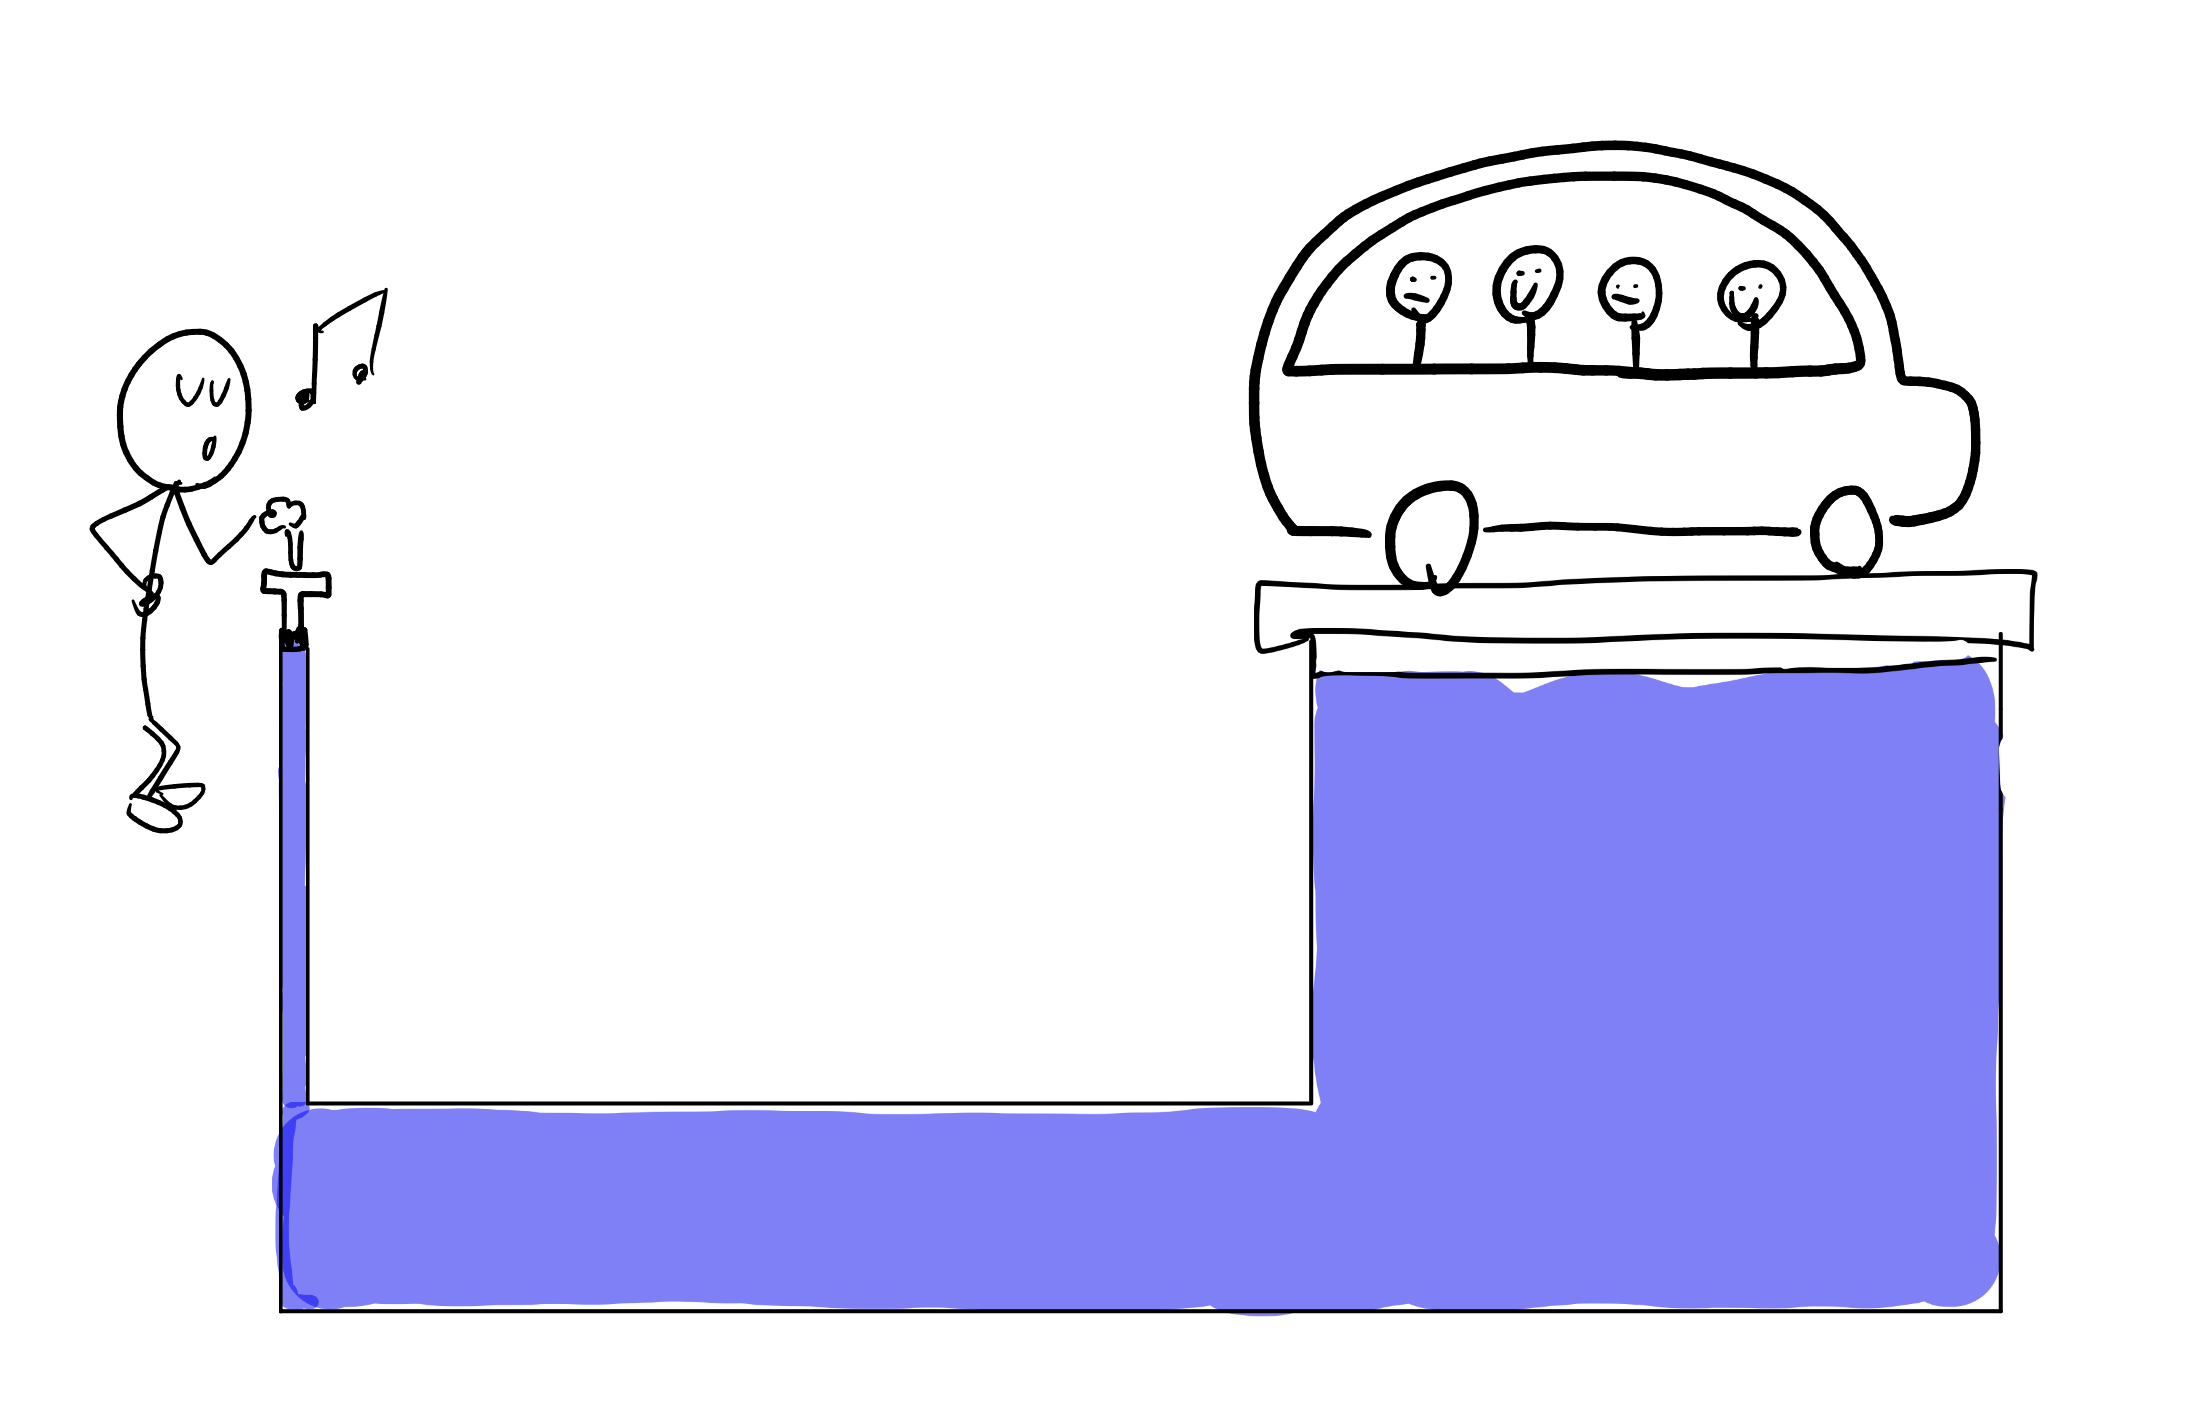
\includegraphics[width=0.85\textwidth]{Images/Kapittel4:Fluiddynamikk/pascal_bil_skisse.png}};
      \begin{scope}[x={(img.south east)}, y={(img.north west)}]
        % Kraften på det lille stempelet (halen i angrepspunktet)
        \draw[->, line width=2.5pt, red!70!black] (0.150,0.591) -- (0.150,0.480);
        \node[right=2pt, red!70!black] at (0.150,0.535) {$\vec{F}_1$};
        \node[anchor=east] at (0.122,0.36) {$A_1$};
        % Trykkøkning i væsken
        \node at (0.342,0.127) {$\Delta p$};
        \node at (0.752,0.326) {$\Delta p$};
        \node at (0.752,0.461) {$A_2$};
        % Kraften fra væsken på det store stempelet: angriper på undersiden,
        % pila er flyttet ut til siden langs den stiplede linjen
        \fill[black] (0.866,0.525) circle (1.8pt);
        \draw[dashed, thick, black!75] (0.866,0.525) -- (0.967,0.525);
        \draw[->, line width=2.5pt, defscol] (0.967,0.525) -- (0.967,0.80);
        \node[above, defscol] at (0.967,0.80) {$\vec{F}_2$};
      \end{scope}
    \end{tikzpicture}
    \caption{Pascals lov i et hydraulisk system. Personen presser lett ned på det lille stempelet (areal \( A_1 \)) med kraften \( \vec{F}_1 \). Trykkøkningen \( \Delta p \) forplanter seg gjennom væsken, og væsken presser opp på det store stempelet (areal \( A_2 \)) med en mye større kraft \( \vec{F}_2 \), som løfter bilen. \( \vec{F}_2 \) virker på undersiden av det store stempelet. Pila er flyttet ut til siden langs den stiplede linjen.}
    \label{fig:pascalslov}
\end{figure}



\exm{Hydraulisk jekk}{%
En hydraulisk jekk har to stempler. Det lille stempelet har areal
$A_1 = \SI{5.0}{\centi\metre\squared} = \SI{5.0e-4}{\metre\squared}$
og det store stempelet har areal
$A_2 = \SI{200}{\centi\metre\squared} = \SI{2.0e-2}{\metre\squared}$.
En kraft $F_1 = \SI{50}{\newton}$ påføres det lille stempelet. Hva er kraften $F_2$ fra væsken på det store stempelet?

\begin{center}
\begin{tikzpicture}[scale=1.0, font=\small, >={Stealth[length=8pt,width=6pt]}]
  % Væske
  \fill[oppgcol!18] (0,0) -- (4.6,0) -- (4.6,1.2) -- (1.6,1.2) -- (1.6,0.4) -- (0.6,0.4) -- (0.6,1.2) -- (0,1.2) -- cycle;
  % Stempler
  \fill[gray!55] (0,1.2) rectangle (0.6,1.4);
  \draw[black!70] (0,1.2) rectangle (0.6,1.4);
  \fill[gray!55] (1.6,1.2) rectangle (4.6,1.4);
  \draw[black!70] (1.6,1.2) rectangle (4.6,1.4);
  % Sylindre
  \draw[very thick, black!75] (0,2.4) -- (0,0) -- (4.6,0) -- (4.6,2.4);
  \draw[very thick, black!75] (0.6,2.4) -- (0.6,0.4) -- (1.6,0.4) -- (1.6,2.4);
  % Krefter (halen i angrepspunktet)
  \draw[->, line width=2.5pt, red!70!black] (0.3,1.4) -- (0.3,0.55);
  \node[font=\small] at (0.3,1.9) {$\vec{F}_1$};
  \draw[->, line width=2.5pt, defscol] (3.1,1.2) -- (3.1,2.9)
      node[right=2pt, font=\small] {$\vec{F}_2$};
  % Arealer
  \node[font=\footnotesize, gray!40!black] at (0.3,2.65) {$A_1$};
  \node[font=\footnotesize, gray!40!black] at (4.1,1.75) {$A_2$};
\end{tikzpicture}
\captionof{figure}{Hydraulisk jekk. Kraften $\vec{F}_1$ virker på det lille stempelet, og væsken presser opp på det store stempelet med kraften $\vec{F}_2$. Figuren er ikke i målestokk.}
\label{fig:hydraulisk_jekk}
\end{center}
}

\svar{%
Fra Pascals lov er trykkøkningen den samme ved begge stemplene:
\[
  \frac{F_1}{A_1} = \frac{F_2}{A_2}
  \implies
  F_2 = F_1 \cdot \frac{A_2}{A_1}
      = \SI{50}{\newton} \cdot \frac{\SI{2.0e-2}{\metre\squared}}{\SI{5.0e-4}{\metre\squared}}
      = \doubleunderline{\SI{2.0e3}{\newton}}
\]
Med et lite stempel kan vi altså løfte en last som er 40 ganger så tung — det er prinsippet bak bilheis og hydrauliske bremser.
}

\oppgaver{Billøfter på verkstedet}{k7oppg5}{%
%
En billøfter på et verksted virker som en hydraulisk jekk. Det lille stempelet har diameter \SI{2.0}{\centi\metre}, og det store stempelet har diameter \SI{20}{\centi\metre}. En bil med masse \SI{1500}{\kilo\gram} står på det store stempelet. Vi ser bort fra massen til stemplene og antar at begge stemplene er i samme høyde.
\begin{enumerate}[a)]
    \item Hvor mange ganger større er arealet av det store stempelet enn arealet av det lille? (Arealet av en sirkel er $A = \pi r^2$.)
    \item Hvor stor kraft må virke på det lille stempelet for å holde bilen oppe?
    \item Det lille stempelet presses \SI{10}{\centi\metre} ned. Hvor mye løftes bilen? \textit{Hint: Væsken som presses ut av den lille sylinderen, må gå inn i den store.}
    \item Regn ut arbeidet som gjøres på det lille stempelet, og arbeidet som gjøres på bilen. Hva ser du? Får vi noe «gratis» med en hydraulisk jekk?
\end{enumerate}
%
%
}

\oppgaver{Hydrauliske bremser}{k7oppg6}{%
%
Når du tråkker på bremsepedalen i en bil, presses et lite stempel inn i en sylinder med bremsevæske. Røret med bremsevæske fører videre til et stempel ved hvert av de fire hjulene. Stempelet ved pedalen har areal \SI{1.5}{\centi\metre\squared}, og hvert av stemplene ved hjulene har areal \SI{9.0}{\centi\metre\squared}. Kraften fra pedalen på det lille stempelet er \SI{200}{\newton}.
\begin{enumerate}[a)]
    \item Finn trykkøkningen i bremsevæsken.
    \item Finn kraften fra bremsevæsken på hvert av stemplene ved hjulene.
    \item Rørene fram til hjulene har ulik lengde. Hvorfor blir likevel kraften på stempelet like stor ved alle fire hjulene?
\end{enumerate}
%
%
}


\section{Oppdrift og Arkimedes' lov}

Når et legeme er omgitt av en væske, utøves en oppdriftskraft på legemet. Denne kraften skyldes at trykket varierer langs legemets høyde. La oss se nærmere på dette. 

Tenk deg et rektangulært legeme med grunnflate $A$ og høyde $h_s$, som er senket helt ned i en væske. Toppen er på dybden $h_1$, og bunnen er på dybden $h_2 = h_1 + h_s$:

\begin{center}
\begin{tikzpicture}[scale=0.95, font=\small, >={Stealth[length=7pt,width=5pt]}]
  % Væske
  \fill[oppgcol!18] (-1.6,-0.4) rectangle (3.4,2.5);
  \draw[oppgcol!70!black, thick] (-1.6,2.5) -- (3.4,2.5) node[right, font=\footnotesize, black!70] {overflate};
  % Legeme
  \fill[headCol!20] (0.2, 0.6) rectangle (2.4, 1.9);
  \draw[thick] (0.2, 0.6) rectangle (2.4, 1.9);
  % Dybder
  \draw[<->, thin, gray!40!black] (-0.4, 2.5) -- (-0.4, 1.9)
      node[midway, left, font=\footnotesize] {$h_1$};
  \draw[<->, thin, gray!40!black] (-1.1, 2.5) -- (-1.1, 0.6)
      node[midway, left, font=\footnotesize] {$h_2$};
  \draw[gray!50, thin, dashed] (-1.2,1.9) -- (0.2,1.9);
  \draw[gray!50, thin, dashed] (-1.2,0.6) -- (0.2,0.6);
  \draw[<->, thin, gray!40!black] (2.7, 1.9) -- (2.7, 0.6)
      node[midway, right, font=\footnotesize] {$h_s$};
  % Krefter (halen i angrepspunktet)
  \draw[->, line width=2.5pt, defscol] (0.7, 1.9) -- (0.7, 1.3)
      node[midway, right=2pt, font=\footnotesize] {$\vec{F}_{\text{topp}}$};
  \draw[->, line width=2.5pt, defscol] (1.9, 0.6) -- (1.9, 1.65)
      node[pos=0.35, left=2pt, font=\footnotesize] {$\vec{F}_{\text{bunn}}$};
\end{tikzpicture}
\captionof{figure}{Trykkreftene på toppen og bunnen av et legeme under vann. Kraften på bunnen er større enn kraften på toppen, fordi trykket er større lenger ned.}
\label{fig:oppdrift_utledning}
\end{center}

\begin{wrapfigure}[6]{r}[1.5cm]{3.6cm}
\vspace{-\baselineskip}%
\rotatebox{-15}{\href{https://youtu.be/euvIlejovCA?si=ZIf3kAZPGtganxjj}{%
\begin{tikzpicture}[inner sep=0pt]
\node[anchor=south west] (thumb) at (0,0) {
\includegraphics[width=3.6cm]{Images/YouTubeLenker/YT_Oppdrift.png}};
\node[anchor=north west] at (thumb.south west) {
\includegraphics[width=1.2cm]{Images/YouTubeLenker/Icon.png}};
\end{tikzpicture}%
}}%
\end{wrapfigure}
Trykkraften \emph{ned} på toppen er $F_{\text{topp}} = p_1\cdot A = (p_0+\rho_v \mathrm{g} h_1)\,A$,
og kraften \emph{opp} på bunnen er $F_{\text{bunn}} = p_2 \cdot A = (p_0+\rho_v \mathrm{g} h_2)\,A$. Merk forøvrig at trykkreftene på sidene er like store fra begge kanter og opphever hverandre.
Kraftsummen fra trykket på legemet kaller vi \emph{oppdriftskraften} $F_{\textrm{B}}$. Bokstaven B står for det engelske ordet \textit{buoyancy}, som betyr oppdrift. Oppdriftskraften er gitt ved:
\[
  F_{\textrm{B}} = F_{\text{bunn}} - F_{\text{topp}}
    = \rho_v \mathrm{g} A (h_2 - h_1)
    = \rho_v \mathrm{g} A h_s
    = \rho_v \mathrm{g} V_\text{f}
\]
Leddet $\rho_v$ er tettheten til væsken, \( \mathrm{g} \) er tyngdeakselerasjonen, og \( V_\text{f} \) er volumet av væsken som fortrenges av legemet. Dermed ser vi at oppdriftskraften \( F_{\textrm{B}} \) er direkte knyttet til vekten av væsken som fortrenges av legemet.

Forskjellen mellom trykkreftene på oversiden og undersiden av legemet gir altså et netto løft, kalt oppdriftskraften \( F_{\textrm{B}} \). 

\defn{Arkimedes' oppdriftslov}{
    Oppdriftskraften \( F_{\textrm{B}} \) på et legeme omgitt av en væske i ro kan uttrykkes som:
    \begin{align}
        F_{\textrm{B}} = \rho_v \mathrm{g} V_\text{f}
    \end{align}
    Her er \( \rho_v \) tettheten til væsken, \( \mathrm{g} \) er tyngdeakselerasjonen, og \( V_\text{f} \) er volumet av væsken under vann. Volumet av legemet i væsken må naturligvis være like stort som volumet av den fortrengte væsken. Dermed ser vi at oppdriftskraften $F_{\textrm{B}}$ er direkte knyttet til tyngden av den fortrengte væsken! 
}

\begin{figure}[H]
    \centering
    \begin{tikzpicture}[scale=1.3, font=\small, >={Stealth[length=8pt,width=6pt]}]
      % Vann og beholder
      \fill[oppgcol!18] (0,0) rectangle (5.0,2.0);
      \draw[oppgcol!70!black, thick] (0,2.0) -- (5.0,2.0);
      \draw[very thick, black!75] (0,3.4) -- (0,0) -- (5.0,0) -- (5.0,3.4);
      % Legeme som flyter
      \fill[headCol!20] (1.6,1.2) rectangle (3.4,2.8);
      \draw[thick, headCol!60!black] (1.6,1.2) rectangle (3.4,2.8);
      \node at (2.5,2.5) {$m$};
      % Dybden h_f
      \draw[<->, thin, gray!40!black] (1.25,1.2) -- (1.25,2.0)
          node[midway, left, font=\footnotesize] {$h_\text{f}$};
      \draw[gray!50, thin] (1.15,1.2) -- (1.6,1.2);
      % Tyngdekraften angriper i massesenteret, oppdriften i sentrum av det
      % fortrengte volumet. Begge ligger på midtlinjen; pilene er skjøvet litt
      % ut til hver side langs stiplede linjer, så de ikke ligger oppå hverandre.
      \draw[dashed, thin, gray!60] (2.5,1.2) -- (2.5,2.8);
      \fill[black] (2.5,2.0) circle (1.8pt);
      \draw[dashed, thick, black!80] (2.5,2.0) -- (2.85,2.0);
      \draw[->, line width=2.5pt, defscol] (2.85,2.0) -- (2.85,0.6)
          node[right=2pt] {$\vec{G}$};
      \fill[black] (2.5,1.6) circle (1.8pt);
      \draw[dashed, thick, black!80] (2.5,1.6) -- (2.15,1.6);
      \draw[->, line width=2.5pt, defscol] (2.15,1.6) -- (2.15,3.0)
          node[left=2pt] {$\vec{F}_{\textrm{B}}$};
    \end{tikzpicture}
    \caption{Et legeme med masse $m$ flyter i vann. Det fortrengte volumet er den delen av legemet som er under vannflaten, $V_\text{f} = h_\text{f}\cdot A$, der $h_\text{f}$ er hvor dypt legemet stikker ned, og $A$ er arealet av bunnflaten. Begge kreftene angriper på legemets midtlinje: oppdriftskraften $\vec{F}_{\textrm{B}}$ i sentrum av det fortrengte volumet og tyngdekraften $\vec{G}$ i massesenteret (prikkene). Pilene er skjøvet litt ut til hver side langs de stiplede linjene, slik at de ikke tegnes oppå hverandre.}
    \label{fig:h-fortrengt}
\end{figure}

\exm{Stein i vann}{%
Du holder en stein i en snor, slik at steinen henger i ro helt under vann. Steinen har masse $m = \SI{5.4}{\kilo\gram}$ og volum $V = \SI{2.0}{\litre}$.
\begin{enumerate}[a)]
    \item Tegn kreftene som virker på steinen.
    \item Finn oppdriftskraften på steinen.
    \item Finn snorkraften $S$. Sammenlign med snorkraften som trengs for å holde steinen i lufta.
\end{enumerate}
}

\svar{%
\noindent
\textbf{a)} Tre krefter virker på steinen: tyngdekraften $\vec{G}$ nedover, oppdriftskraften $\vec{F}_{\textrm{B}}$ oppover og snorkraften $\vec{S}$ oppover.

\begin{center}
\begin{tikzpicture}[scale=1.0, font=\small, >={Stealth[length=8pt,width=6pt]}]
  \fill[oppgcol!18] (-2.0,-2.2) rectangle (2.0,1.9);
  \draw[oppgcol!70!black, thick] (-2.0,1.9) -- (2.0,1.9);
  \draw[black!70, thick] (0,0.7) -- (0,2.6);
  \fill[gray!55] (0,0) ellipse (0.95 and 0.7);
  \draw[gray!30!black] (0,0) ellipse (0.95 and 0.7);
  % Krefter (halen i angrepspunktet)
  \draw[->, line width=2.5pt, defscol] (0,0.7) -- (0,1.75)
      node[right=2pt, font=\small] {$\vec{S}$};
  % G og F_{\textrm{B}} angriper i samme punkt (sentrum); stiplede linjer flytter pilene til siden
  \draw[dashed, thick, black!75] (-0.6,0) -- (0.6,0);
  \fill[black] (0,0) circle (1.8pt);
  \draw[->, line width=2.5pt, defscol] (0.6,0) -- (0.6,-1.75)
      node[right=2pt, font=\small] {$\vec{G}$};
  \draw[->, line width=2.5pt, defscol] (-0.6,0) -- (-0.6,0.65)
      node[left=2pt, font=\small] {$\vec{F}_{\textrm{B}}$};
\end{tikzpicture}
\captionof{figure}{Kreftene som virker på steinen. $\vec{G}$ og $\vec{F}_{\textrm{B}}$ angriper begge i sentrum av steinen (prikken). Pilene er flyttet ut til hver sin side langs den stiplede linjen, slik at de ikke tegnes oppå hverandre.}
\label{fig:stein_i_vann}
\end{center}

\noindent
\textbf{b)} Steinen er helt under vann, så det fortrengte volumet er hele steinens volum, $V_\text{f} = \SI{2.0}{\litre} = \SI{2.0e-3}{\metre\cubed}$:
\[
    F_{\textrm{B}} = \rho_v\mathrm{g}V_\text{f} = \SI{1000}{\kilo\gram\per\metre\cubed}\cdot\SI{9.81}{\metre\per\second\squared}\cdot\SI{2.0e-3}{\metre\cubed} = \SI{19.6}{\newton} \approx \doubleunderline{\SI{20}{\newton}}
\]

\smallskip\noindent
\textbf{c)} Steinen er i ro, så $\sum F = 0$. Med positiv retning oppover:
\[
    S + F_{\textrm{B}} - G = 0 \quad\implies\quad S = G - F_{\textrm{B}}
\]
Tyngdekraften er $G = m\mathrm{g} = \SI{5.4}{\kilo\gram}\cdot\SI{9.81}{\metre\per\second\squared} = \SI{53.0}{\newton}$, så
\[
    S = \SI{53.0}{\newton} - \SI{19.6}{\newton} = \SI{33.4}{\newton} \approx \doubleunderline{\SI{33}{\newton}}
\]
I lufta må snora holde hele tyngden, \SI{53}{\newton} (oppdriften i luft er så liten at vi kan se bort fra den). Under vann trenger snora bare å holde \SI{33}{\newton}. Derfor føles steiner lettere når vi løfter dem under vann.
}


For å avgjøre om et legeme flyter eller synker, må vi sammenligne oppdriftskraften med tyngdekraften på legemet. Tyngdekraften \( G \) avhenger av legemets masse \( m \) og tyngdeakselerasjonen \( \mathrm{g} \). Hvis massen til legemet uttrykkes som \( m = \rho_L V \), der \( \rho_L \) er legemets tetthet og \( V \) er volumet, kan tyngdekraften skrives som:
\[
G = m \mathrm{g} = \rho_L V \mathrm{g}.
\]
Nå har vi både oppdriftskraften og tyngdekraften uttrykt ved tettheter og volum. Det gjør det lett å sammenligne dem.

Nettokraften på et legeme med tetthet $\rho_L$ og volum $V$ helt nedsenket i en væske med tetthet $\rho_v$ er:
\[
  F_{\text{netto}} = F_{\textrm{B}} - G = \rho_v \mathrm{g} V - \rho_L \mathrm{g} V = (\rho_v - \rho_L)\,\mathrm{g} V
\]

\begin{tcolorbox}[colback=gray!13, colframe=gray!40, boxrule=0.5pt,
    arc=2pt, left=6pt, right=6pt, top=4pt, bottom=4pt]
\begin{itemize}
  \item $\rho_L < \rho_v$: $F_{\text{netto}} > 0$ — legemet \textbf{flyter} (akselererer opp til det er delvis ute av væsken).
  \item $\rho_L = \rho_v$: $F_{\text{netto}} = 0$ — legemet \textbf{svever} i likevekt inne i væsken.
  \item $\rho_L > \rho_v$: $F_{\text{netto}} < 0$ — legemet \textbf{synker}.
\end{itemize}
\end{tcolorbox}

Når et legeme flyter i ro på overflaten, er bare en del av det under væsken. Da er oppdriftskraften akkurat like stor som tyngdekraften, $F_{\textrm{B}} = G$.

\merk{Stål flyter ikke i vann — men et stålskip gjør det!}{%
Stål har tetthet $\rho \approx \SI{7850}{\kilo\gram\per\metre\cubed}$, langt høyere enn vann.
Likevel flyter et skip laget av stål, fordi \emph{skipet som helhet} — stål pluss luft inni —
har en gjennomsnittlig tetthet \emph{lavere} enn vann.
Det er den totale massen delt på det totale volumet som avgjør.}

\exm{Toppen av isfjellet}{%
Et isfjell flyter i sjøen. Hvor stor andel av isfjellet ligger under vann? Bruk tettheter fra tabell~\ref{tab:massetetthet}.
}

\svar{%
Isfjellet flyter i ro, så oppdriftskraften er like stor som tyngdekraften:
\[
    F_{\textrm{B}} = G
\]
La $V$ være hele volumet til isfjellet og $V_\text{f}$ volumet som er under vann. Vi setter inn uttrykkene for $F_{\textrm{B}}$ og $G$:
\[
    \rho_\text{sjø}\,\mathrm{g}\,V_\text{f} = \rho_\text{is}\,\mathrm{g}\,V
\]
Vi deler på $\mathrm{g}$ og på $V$ på begge sider og får
\[
    \frac{V_\text{f}}{V} = \frac{\rho_\text{is}}{\rho_\text{sjø}} = \frac{\SI{0.92e3}{\kilo\gram\per\metre\cubed}}{\SI{1.03e3}{\kilo\gram\per\metre\cubed}} = 0.893 \approx \doubleunderline{\SI{89}{\percent}}
\]
Omtrent ni tideler av isfjellet ligger altså under vann, og bare én tidel stikker opp. Det er derfor vi sier at noe bare er «toppen av isfjellet».
}

\exm{Oppdrift på en båt}{%
En båt har et volum på \( V = 9.0 \, \text{m}^3 \), og \( 12\% \) av dette volumet er under vann.
\begin{enumerate}[a)]
    \item Hva er oppdriftskraften på båten?
    \item Hva er massen til båten?
\end{enumerate}
}

\svar{%
\noindent
\textbf{a)} Volumet av vann som fortrenges er:
\[
V_\text{f} = 0.12 \cdot V = 0.12 \cdot 9.0 \, \text{m}^3 = 1.08 \, \text{m}^3.
\]
Oppdriftskraften beregnes ved å bruke formelen for oppdrift:
\[
F_{\textrm{B}} = \rho_v \mathrm{g} V_\text{f} = 1000 \, \text{kg/m}^3 \cdot 9.81 \, \text{m/s}^2 \cdot 1.08 \, \text{m}^3 = 10594.8 \, \text{N} \approx \doubleunderline{11 \, \text{kN}}.
\]

\smallskip\noindent
\textbf{b)} Når båten flyter, er oppdriftskraften lik tyngdekraften på båten:
\[
F_{\textrm{B}} = G = m \mathrm{g}.
\]
Vi løser for massen \( m \):
\[
m = \frac{F_{\textrm{B}}}{\mathrm{g}} = \frac{10594.8 \, \text{N}}{9.81 \, \text{m/s}^2} = 1080 \, \text{kg} \approx \doubleunderline{1.1 \cdot 10^3 \, \text{kg}}.
\]
Legg merke til at båtens masse er lik massen til vannet den fortrenger, $\rho_v V_\text{f} = \SI{1080}{\kilo\gram}$. Det er nettopp det Arkimedes' lov sier.
}

\exm{Stein, båt og basseng}{%
En liten båt flyter i et basseng. I båten ligger en stein med masse $m_\text{s} = \SI{3.0}{\kilo\gram}$ og massetetthet $\rho_\text{s} = \SI{2.5e3}{\kilo\gram\per\metre\cubed}$. Vannflaten i bassenget har areal $A = \SI{2.0}{\metre\squared}$. Du tar steinen ut av båten og slipper den ned i bassenget, der den synker til bunnen (se figuren).

Når står vannet høyest i bassenget: når steinen ligger i båten, eller når steinen ligger på bunnen av bassenget?
\begin{enumerate}[a)]
    \item Finn volumet av vann som fortrenges på grunn av steinen når steinen ligger i båten.
    \item Finn volumet av vann som fortrenges på grunn av steinen når den ligger på bunnen.
    \item Hvor mye høyere står vannet i det ene tilfellet enn i det andre?
\end{enumerate}

\begin{center}
\begin{tikzpicture}[scale=0.9, font=\small]
  % ---- (a) Steinen i båten ----
  \begin{scope}
    \fill[oppgcol!18] (0,0) rectangle (4.5,1.6);
    \draw[oppgcol!70!black, thick] (0,1.6) -- (4.5,1.6);
    \draw[very thick, black!75] (0,2.6) -- (0,0) -- (4.5,0) -- (4.5,2.6);
    % Båt (lavt i vannet)
    \fill[headCol!45] (1.2,1.95) -- (3.3,1.95) -- (3.0,1.25) -- (1.5,1.25) -- cycle;
    \draw[thick, headCol!70!black] (1.2,1.95) -- (3.3,1.95) -- (3.0,1.25) -- (1.5,1.25) -- cycle;
    % Stein i båten
    \fill[gray!60] (2.25,2.13) ellipse (0.32 and 0.18);
    \draw[gray!30!black] (2.25,2.13) ellipse (0.32 and 0.18);
    \node[font=\small] at (2.25,-0.35) {(a) Steinen i båten};
  \end{scope}
  % ---- (b) Steinen på bunnen ----
  \begin{scope}[xshift=5.5cm]
    \fill[oppgcol!18] (0,0) rectangle (4.5,1.4);
    \draw[oppgcol!70!black, thick] (0,1.4) -- (4.5,1.4);
    \draw[very thick, black!75] (0,2.6) -- (0,0) -- (4.5,0) -- (4.5,2.6);
    % Båt (høyere i vannet)
    \fill[headCol!45] (1.2,1.95) -- (3.3,1.95) -- (3.0,1.25) -- (1.5,1.25) -- cycle;
    \draw[thick, headCol!70!black] (1.2,1.95) -- (3.3,1.95) -- (3.0,1.25) -- (1.5,1.25) -- cycle;
    % Stein på bunnen
    \fill[gray!60] (3.6,0.18) ellipse (0.32 and 0.18);
    \draw[gray!30!black] (3.6,0.18) ellipse (0.32 and 0.18);
    \node[font=\small] at (2.25,-0.35) {(b) Steinen på bunnen};
  \end{scope}
  % Vannstanden i (a) som referanse
  \draw[dashed, gray!60!black] (4.5,1.6) -- (10.0,1.6);
  \node[right, font=\footnotesize] at (10.0,1.6) {?};
\end{tikzpicture}
\captionof{figure}{En båt med en stein flyter i et basseng. (a) Steinen ligger i båten. (b) Steinen er sluppet ned i bassenget og ligger på bunnen. Den stiplede linjen viser vannstanden i (a). Figuren er ikke i målestokk.}
\label{fig:stein_baat_basseng}
\end{center}
}

\svar{%
\noindent
Båten fortrenger like mye vann på grunn av sin egen masse i begge tilfellene. Vi trenger derfor bare å se på hvor mye vann som fortrenges på grunn av \emph{steinen}.

\smallskip\noindent
\textbf{a)} Når steinen ligger i båten, flyter båten og steinen sammen. Da er oppdriftskraften lik tyngden: $F_{\textrm{B}} = G$. Den ekstra oppdriftskraften som trengs for å bære steinen, er lik tyngden av steinen:
\[
    \rho_v\mathrm{g}V_1 = m_\text{s}\mathrm{g}
    \quad\implies\quad
    V_1 = \frac{m_\text{s}}{\rho_v} = \frac{\SI{3.0}{\kilo\gram}}{\SI{1.0e3}{\kilo\gram\per\metre\cubed}} = \doubleunderline{\SI{3.0e-3}{\metre\cubed}}
\]
Båten må altså fortrenge vann med \emph{samme masse} som steinen, \SI{3.0}{\litre}.

\smallskip\noindent
\textbf{b)} Når steinen ligger på bunnen, fortrenger den bare sitt eget volum:
\[
    V_2 = \frac{m_\text{s}}{\rho_\text{s}} = \frac{\SI{3.0}{\kilo\gram}}{\SI{2.5e3}{\kilo\gram\per\metre\cubed}} = \doubleunderline{\SI{1.2e-3}{\metre\cubed}}
\]
Det er bare \SI{1.2}{\litre}, fordi steinen har større massetetthet enn vann.

\smallskip\noindent
\textbf{c)} Når et volum $V$ vann blir fortrengt, stiger vannflaten med $\Delta h = V/A$. Forskjellen i vannstand er derfor
\[
    \Delta h = \frac{V_1 - V_2}{A} = \frac{\SI{3.0e-3}{\metre\cubed} - \SI{1.2e-3}{\metre\cubed}}{\SI{2.0}{\metre\squared}} = \SI{9.0e-4}{\metre} = \doubleunderline{\SI{0.90}{\milli\metre}}
\]
Vannet står altså \doubleunderline{høyest når steinen ligger i båten}. Når du slipper steinen ned i bassenget, synker vannstanden litt. Grunnen er at en flytende stein må fortrenge vann med like stor \emph{masse} som seg selv, mens en stein på bunnen bare fortrenger vann med like stort \emph{volum} som seg selv.
}

\subsection{Ekstra: Løft på flyvinger og propeller}

Oppdriftskraften skyldes at trykket på undersiden av et legeme er større enn trykket på oversiden. Det samme prinsippet, at en trykkforskjell gir en netto kraft, forklarer også hvordan en flyvinge holder et fly oppe. Forskjellen er at trykkforskjellen nå ikke skyldes dybden, men at lufta \emph{strømmer} rundt vingen.

Et tverrsnitt av en flyvinge kalles en \emph{vingeprofil} (på engelsk \textit{airfoil}). Profilen er avrundet foran, spiss bak, og som regel mer krummet på oversiden enn på undersiden. I tillegg er vingen gjerne vinklet litt opp i forkant. Når flyet beveger seg framover, strømmer lufta rundt vingen. Formen og vinkelen gjør at lufta over vingen strømmer \emph{fortere} enn lufta under, og at lufta bøyes nedover bak vingen. Akkurat som i det smale røret i figur~\ref{fig:roer_variabelt_areal} gjelder det at der lufta strømmer fortere, er trykket lavere. Trykket på oversiden av vingen blir derfor lavere enn trykket på undersiden.

\begin{center}
\begin{tikzpicture}[scale=1.0, font=\small, >={Stealth[length=7pt,width=5pt]}]
  % Strømlinjer: tettere over vingen (større fart), bøyes nedover bak vingen
  \foreach \y/\e in {2.3/0.9, 1.6/0.35, 0.95/-0.25} {
    \draw[->, oppgcol!80!black, thin] (-1.8,\y) .. controls (0.3,\y+0.35) and (3.2,\y+0.2) .. (7.8,\e);
  }
  \foreach \y/\e in {-0.6/-1.2, -1.3/-1.75} {
    \draw[->, oppgcol!80!black, thin] (-1.8,\y) .. controls (1.5,\y) and (4.0,\y-0.1) .. (7.8,\e);
  }
  % Vingeprofil (litt vinklet opp i forkant)
  \begin{scope}[rotate=-6]
    \fill[headCol!20] (0,0) .. controls (0.05,0.75) and (2.2,0.95) .. (6,0.05)
                  .. controls (3.8,-0.2) and (0.6,-0.45) .. (0,0) -- cycle;
    \draw[thick, headCol!60!black] (0,0) .. controls (0.05,0.75) and (2.2,0.95) .. (6,0.05)
                  .. controls (3.8,-0.2) and (0.6,-0.45) .. (0,0) -- cycle;
  \end{scope}
  % Luftstrøm inn
  \draw[->, thick, black!70] (-3.2,0.1) -- (-2.1,0.1);
  \node[font=\footnotesize, black!70] at (-2.65,0.45) {luftstrøm};
  % Trykk
  \node[font=\footnotesize, align=center] at (3.8,3.15) {lavere trykk, $p_\text{over}$ (større fart)};
  \node[font=\footnotesize, align=center] at (3.8,-2.35) {høyere trykk, $p_\text{under}$};
  % Løft (halen i vingen)
  \draw[->, line width=2.5pt, defscol] (2.4,0.1) -- (2.4,2.0) node[right=3pt, pos=0.85, font=\small] {$\vec{F}_\text{L}$};
\end{tikzpicture}
\captionof{figure}{Tverrsnitt av en flyvinge med strømlinjer. Lufta strømmer fortere over vingen enn under (strømlinjene ligger tettere), og trykket over vingen blir lavere enn trykket under. Trykkforskjellen gir en netto kraft oppover: løftet $\vec{F}_\text{L}$.}
\label{fig:vingeprofil}
\end{center}

Akkurat som for oppdriftskraften får vi altså en netto kraft oppover, fordi lufta presser hardere på undersiden enn på oversiden. Denne kraften kalles \emph{løftet} $F_\text{L}$ (L for det engelske \textit{lift}). Er trykkforskjellen $\Delta p = p_\text{under} - p_\text{over}$ og vingearealet $A$, er løftet omtrent
\[
  F_\text{L} \approx \Delta p \cdot A
\]
Trykkforskjellen trenger ikke være stor. Et lite fly med masse \SI{1.0e3}{\kilo\gram} og vingeareal \SI{16}{\metre\squared} holdes oppe i jevn flukt når $F_\text{L} = G$. Det gir $\Delta p = m\mathrm{g}/A = \SI{9.81e3}{\newton}/\SI{16}{\metre\squared} \approx \SI{6.1e2}{\pascal}$. Det er under én prosent av lufttrykket!

\merk{En vanlig misforståelse}{Det sies ofte at lufta over og under vingen må bruke like lang tid fra forkanten til bakkanten, og at lufta over derfor må gå fortere fordi veien er lengre. Det stemmer ikke. Lufta over vingen kommer faktisk fram til bakkanten \emph{før} lufta under. Det er formen og vinkelen på vingen som bestemmer hvordan lufta strømmer. Vingen bøyer lufta nedover, og etter Newtons tredje lov dytter lufta da vingen oppover. Trykkforskjellen og nedbøyingen av lufta er to sider av samme sak.}

En \emph{propell} virker på samme måte. Hvert propellblad er en liten vinge som roterer. Bladet har en vingeprofil, men er vendt slik at «oversiden» peker framover. Når propellen roterer, strømmer lufta fortere over den fremre siden av bladet, og trykket der blir lavere enn på baksiden. Trykkforskjellen gir en kraft framover, som vi kaller \emph{skyvekraften}. Den trekker flyet framover. Det samme prinsippet brukes i båtpropeller, vifter, helikopterrotorer og vindturbiner.

\begin{center}
\begin{tikzpicture}[scale=0.9, font=\small, >={Stealth[length=7pt,width=5pt]}]
  % (a) Propell sett forfra
  \begin{scope}
    \fill[headCol!20] (0,0) .. controls (0.45,0.6) and (0.5,1.9) .. (0.15,2.6)
                       .. controls (-0.1,2.7) and (-0.35,2.0) .. (-0.3,0.6) -- cycle;
    \draw[thick, headCol!60!black] (0,0) .. controls (0.45,0.6) and (0.5,1.9) .. (0.15,2.6)
                       .. controls (-0.1,2.7) and (-0.35,2.0) .. (-0.3,0.6) -- cycle;
    \begin{scope}[rotate=180]
    \fill[headCol!20] (0,0) .. controls (0.45,0.6) and (0.5,1.9) .. (0.15,2.6)
                       .. controls (-0.1,2.7) and (-0.35,2.0) .. (-0.3,0.6) -- cycle;
    \draw[thick, headCol!60!black] (0,0) .. controls (0.45,0.6) and (0.5,1.9) .. (0.15,2.6)
                       .. controls (-0.1,2.7) and (-0.35,2.0) .. (-0.3,0.6) -- cycle;
    \end{scope}
    \fill[black!60] (0,0) circle (0.28);
    % Rotasjonsretning
    \draw[->, thick, black!70] (1.25,-0.9) arc (-40:40:1.5);
    % Snitt
    \draw[dashed, thick, black!70] (-0.9,1.6) -- (1.0,1.6) node[right, font=\footnotesize] {snitt};
    \node at (0,-3.2) {(a) Propell sett forfra};
  \end{scope}
  % (b) Tverrsnitt av bladet sett fra siden (flyet flyr mot venstre).
  % Bladet beveger seg nedover, så forkanten er nederst. Den krumme siden vender framover.
  \begin{scope}[xshift=6.4cm, yshift=0cm]
    \begin{scope}[shift={(0,-1.9)}, rotate=78]
      \fill[headCol!20] (0,0) .. controls (0.05,0.6) and (1.5,0.75) .. (4,0.05)
                  .. controls (2.5,-0.15) and (0.4,-0.35) .. (0,0) -- cycle;
      \draw[thick, headCol!60!black] (0,0) .. controls (0.05,0.6) and (1.5,0.75) .. (4,0.05)
                  .. controls (2.5,-0.15) and (0.4,-0.35) .. (0,0) -- cycle;
    \end{scope}
    % Bladets bevegelse
    \draw[->, thick, black!70] (1.5,1.2) -- (1.5,-0.2);
    \node[font=\footnotesize, align=left, right] at (1.6,0.5) {bladet\\beveger seg};
    \node[font=\footnotesize, align=center] at (-2.0,1.3) {lavere\\trykk};
    \node[font=\footnotesize, align=center] at (1.6,-1.6) {høyere\\trykk};
    % Skyvekraft (halen i bladet, peker framover = mot venstre)
    \draw[->, line width=2.5pt, defscol] (-0.05,-0.3) -- (-1.9,-0.3) node[below=2pt, font=\small] {$\vec{F}_\text{skyv}$};
    \draw[->, thick, black!70] (-2.9,2.6) -- (-4.1,2.6);
    \node[font=\footnotesize] at (-3.5,2.95) {flyets fartsretning};
    \node at (-0.6,-3.2) {(b) Tverrsnitt av ett blad};
  \end{scope}
\end{tikzpicture}
\captionof{figure}{(a) En propell sett forfra. Bladene roterer, og hvert blad har en vingeprofil. (b) Tverrsnitt av ett blad, sett fra siden. Flyet beveger seg mot venstre, og bladet beveger seg nedover i figuren. Trykket er lavere på den fremre siden av bladet enn på baksiden. Trykkforskjellen gir skyvekraften $\vec{F}_\text{skyv}$, som peker framover.}
\label{fig:propell}
\end{center}

\oppgaver{Er kronen av gull?}{k7oppg7}{%
%
Ifølge en gammel fortelling fikk Arkimedes i oppdrag av kongen å finne ut om en ny krone var laget av rent gull. Vi gjør et tilsvarende forsøk. En krone har masse \SI{1.00}{\kilo\gram}. Vi henger kronen i en kraftmåler og senker den helt ned i vann. Mens kronen henger i ro under vann, viser kraftmåleren \SI{9.15}{\newton}.
\begin{enumerate}[a)]
    \item Tegn kreftene som virker på kronen mens den henger under vann.
    \item Finn oppdriftskraften på kronen.
    \item Finn volumet til kronen.
    \item Finn massetettheten til kronen. Er den laget av rent gull?
\end{enumerate}
%
%
}

\oppgaver{Trekloss som flyter}{k7oppg8}{%
%
En rektangulær trekloss er \SI{20}{\centi\metre} lang, \SI{10}{\centi\metre} bred og \SI{10}{\centi\metre} høy. Treet har massetetthet \SI{600}{\kilo\gram\per\metre\cubed}. Klossen legges i vann, der den flyter med den største flaten ned.
\begin{enumerate}[a)]
    \item Finn massen til klossen.
    \item Hvor stor andel av klossens volum er under vann?
    \item Hvor dypt stikker klossen ned i vannet?
    \item Hvor stor masse kan du legge oppå klossen før den synker helt ned under vannflaten?
\end{enumerate}
%
%
}


\clearpage
\section{Ekstraoppgaver}

Her er flere oppgaver fra temaene vi har behandlet i dette kapitlet.

\oppgaver{Lufta i et klasserom}{k7oppg9}{%
%
Et klasserom er \SI{5.0}{\metre} langt, \SI{4.0}{\metre} bredt og \SI{2.5}{\metre} høyt. Lufta har massetetthet \SI{1.2}{\kilo\gram\per\metre\cubed}.
\begin{enumerate}[a)]
    \item Finn massen til lufta i klasserommet.
    \item Sammenlign med massen til en voksen person. Er svaret overraskende?
\end{enumerate}
%
%
}

\oppgaver{Dykking i sjøen}{k7oppg10}{%
%
En dykker svømmer \SI{30}{\metre} under overflaten i sjøen. Sjøvann har massetetthet \SI{1030}{\kilo\gram\per\metre\cubed}, og lufttrykket ved overflaten er $p_0 = \SI{1.013e5}{\pascal}$.
\begin{enumerate}[a)]
    \item Finn det totale trykket på dykkeren.
    \item Hvor mange ganger større er dette trykket enn lufttrykket ved overflaten?
\end{enumerate}
%
%
}

\oppgaver{Sugerør}{k7oppg11}{%
%
Når du drikker med sugerør, senker du trykket i munnen. Da er det lufttrykket på væskeoverflaten i glasset som presser væsken opp i sugerøret.
\begin{enumerate}[a)]
    \item Tenk deg at du klarer å fjerne all lufta i sugerøret, slik at trykket over vannet i røret blir null. Hvor høyt kan lufttrykket da presse vannet opp i røret? Lufttrykket er $p_0 = \SI{1.013e5}{\pascal}$.
    \item Kan man drikke vann med et \SI{12}{\metre} langt sugerør, uansett hvor kraftig man suger? Begrunn svaret.
\end{enumerate}
%
%
}

\oppgaver{Vindu i en ubåt}{k7oppg12}{%
%
En ubåt ligger \SI{100}{\metre} under overflaten i sjøen ($\rho = \SI{1030}{\kilo\gram\per\metre\cubed}$). Inne i ubåten er trykket det samme som lufttrykket ved overflaten. Ubåten har et vindu med areal \SI{0.050}{\metre\squared}.
\begin{enumerate}[a)]
    \item Finn trykkforskjellen mellom utsiden og innsiden av vinduet.
    \item Finn nettokraften fra vannet og lufta på vinduet.
\end{enumerate}
\textit{Hint: Lufttrykket virker både på overflaten av sjøen og inne i ubåten.}
%
%
}

\oppgaver{Heliumballong}{k7oppg13}{%
%
Arkimedes' lov gjelder ikke bare i væsker, men også i gasser. En ballong er fylt med \SI{0.010}{\metre\cubed} helium. Helium har massetetthet \SI{0.18}{\kilo\gram\per\metre\cubed}, og lufta rundt har massetetthet \SI{1.2}{\kilo\gram\per\metre\cubed}. Selve ballongen (gummien og snora) har masse \SI{3.0}{\gram}. Vi ser bort fra volumet til gummien.
\begin{enumerate}[a)]
    \item Finn oppdriftskraften fra lufta på ballongen.
    \item Finn tyngdekraften på ballongen med helium.
    \item Vil ballongen stige eller synke? Finn nettokraften på ballongen.
\end{enumerate}
%
%
}

\oppgaver{Olje og vann i et U-rør}{k7oppg14}{%
%
Et U-rør inneholder vann. I det venstre røret heller vi oppå vannet en \SI{10.0}{\centi\metre} høy søyle med olje, som har massetetthet \SI{800}{\kilo\gram\per\metre\cubed}. Olje og vann blander seg ikke. Når alt står i ro, ligger grenseflaten mellom olje og vann i den venstre delen av røret (se figuren).

\begin{center}
\begin{tikzpicture}[scale=0.9, font=\small]
  % Vann
  \fill[oppgcol!25] (0,0) -- (2.6,0) -- (2.6,1.8) -- (2.0,1.8) -- (2.0,0.6) -- (0.6,0.6) -- (0.6,1.0) -- (0,1.0) -- cycle;
  % Olje
  \fill[yellow!45!orange!40] (0,1.0) rectangle (0.6,2.0);
  % Rør
  \draw[very thick, black!75] (0,3.0) -- (0,0) -- (2.6,0) -- (2.6,3.0);
  \draw[very thick, black!75] (0.6,3.0) -- (0.6,0.6) -- (2.0,0.6) -- (2.0,3.0);
  % Nivålinje ved grenseflaten
  \draw[dashed, gray!60!black] (-0.3,1.0) -- (2.9,1.0);
  \fill[black] (0.3,1.0) circle (1.8pt) node[below right=-1pt, font=\footnotesize] {A};
  \fill[black] (2.3,1.0) circle (1.8pt) node[below right=-1pt, font=\footnotesize] {B};
  % Etiketter
  \draw[thin, black!60] (0.45,1.7) -- (1.2,2.3) node[right, font=\footnotesize] {olje};
  \node[right, font=\footnotesize] at (2.7,1.4) {vann};
  \draw[<->, thin, gray!40!black] (-0.3,1.0) -- (-0.3,2.0)
      node[midway, left, font=\footnotesize] {\SI{10.0}{\centi\metre}};
\end{tikzpicture}
\end{center}

\begin{enumerate}[a)]
    \item Punkt A ligger ved grenseflaten mellom olje og vann i det venstre røret, og punkt B ligger i samme høyde i det høyre røret. Forklar hvorfor trykket i A og B er likt.
    \item Hvor høyt over grenseflaten står vannet i det høyre røret?
    \item Hvor mye høyere står oljeoverflaten enn vannoverflaten?
\end{enumerate}
%
%
}
